% Created by tikzDevice version 0.12.3.1 on 2021-03-01 22:37:21
% !TEX encoding = UTF-8 Unicode
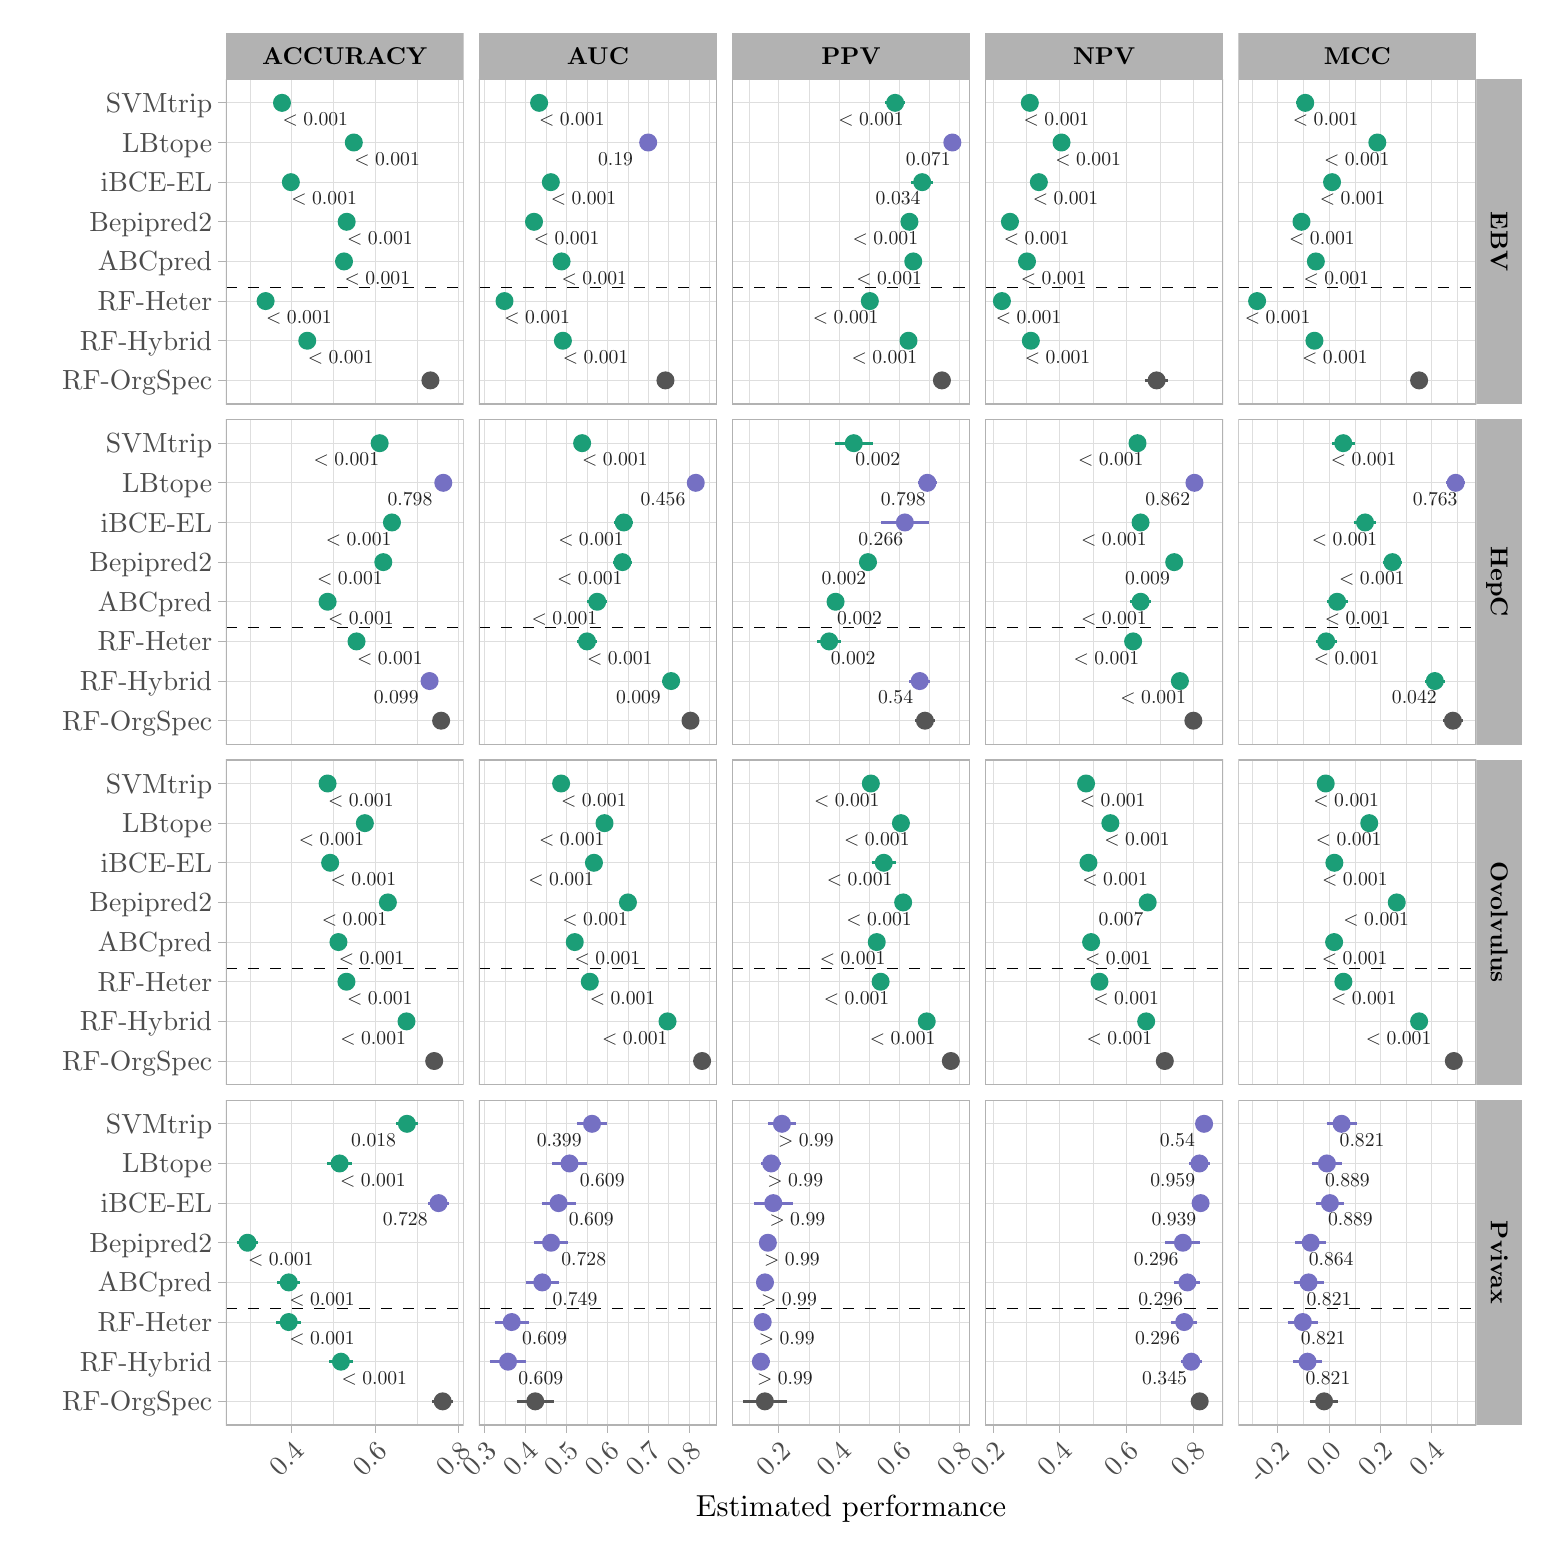
\begin{tikzpicture}[x=1pt,y=1pt]
\definecolor{fillColor}{RGB}{255,255,255}
\path[use as bounding box,fill=fillColor,fill opacity=0.00] (0,0) rectangle (542.02,542.02);
\begin{scope}
\path[clip] (  0.00,  0.00) rectangle (542.02,542.02);
\definecolor{drawColor}{RGB}{255,255,255}
\definecolor{fillColor}{RGB}{255,255,255}

\path[draw=drawColor,line width= 0.6pt,line join=round,line cap=round,fill=fillColor] ( -0.00,  0.00) rectangle (542.02,542.02);
\end{scope}
\begin{scope}
\path[clip] ( 71.60,405.97) rectangle (157.56,523.44);
\definecolor{fillColor}{RGB}{255,255,255}

\path[fill=fillColor] ( 71.60,405.97) rectangle (157.56,523.44);
\definecolor{drawColor}{gray}{0.87}

\path[draw=drawColor,line width= 0.1pt,line join=round] ( 80.37,405.97) --
	( 80.37,523.44);

\path[draw=drawColor,line width= 0.1pt,line join=round] (110.47,405.97) --
	(110.47,523.44);

\path[draw=drawColor,line width= 0.1pt,line join=round] (140.57,405.97) --
	(140.57,523.44);

\path[draw=drawColor,line width= 0.3pt,line join=round] ( 71.60,414.56) --
	(157.56,414.56);

\path[draw=drawColor,line width= 0.3pt,line join=round] ( 71.60,428.89) --
	(157.56,428.89);

\path[draw=drawColor,line width= 0.3pt,line join=round] ( 71.60,443.22) --
	(157.56,443.22);

\path[draw=drawColor,line width= 0.3pt,line join=round] ( 71.60,457.54) --
	(157.56,457.54);

\path[draw=drawColor,line width= 0.3pt,line join=round] ( 71.60,471.87) --
	(157.56,471.87);

\path[draw=drawColor,line width= 0.3pt,line join=round] ( 71.60,486.19) --
	(157.56,486.19);

\path[draw=drawColor,line width= 0.3pt,line join=round] ( 71.60,500.52) --
	(157.56,500.52);

\path[draw=drawColor,line width= 0.3pt,line join=round] ( 71.60,514.85) --
	(157.56,514.85);

\path[draw=drawColor,line width= 0.3pt,line join=round] ( 95.42,405.97) --
	( 95.42,523.44);

\path[draw=drawColor,line width= 0.3pt,line join=round] (125.52,405.97) --
	(125.52,523.44);

\path[draw=drawColor,line width= 0.3pt,line join=round] (155.62,405.97) --
	(155.62,523.44);
\definecolor{drawColor}{RGB}{85,85,85}

\path[draw=drawColor,line width= 1.1pt,line join=round] (143.28,414.56) -- (147.79,414.56);
\definecolor{drawColor}{RGB}{27,158,119}

\path[draw=drawColor,line width= 1.1pt,line join=round] ( 98.55,428.89) -- (103.50,428.89);

\path[draw=drawColor,line width= 1.1pt,line join=round] ( 83.74,443.22) -- ( 88.21,443.22);

\path[draw=drawColor,line width= 1.1pt,line join=round] (111.97,457.54) -- (116.65,457.54);

\path[draw=drawColor,line width= 1.1pt,line join=round] (112.83,471.87) -- (117.72,471.87);

\path[draw=drawColor,line width= 1.1pt,line join=round] ( 92.65,486.19) -- ( 97.55,486.19);

\path[draw=drawColor,line width= 1.1pt,line join=round] (115.41,500.52) -- (120.26,500.52);

\path[draw=drawColor,line width= 1.1pt,line join=round] ( 89.46,514.85) -- ( 94.34,514.85);
\definecolor{drawColor}{RGB}{85,85,85}
\definecolor{fillColor}{RGB}{85,85,85}

\path[draw=drawColor,line width= 0.8pt,line join=round,line cap=round,fill=fillColor] (145.53,414.56) circle (  2.85);
\definecolor{drawColor}{RGB}{27,158,119}
\definecolor{fillColor}{RGB}{27,158,119}

\path[draw=drawColor,line width= 0.8pt,line join=round,line cap=round,fill=fillColor] (101.03,428.89) circle (  2.85);

\path[draw=drawColor,line width= 0.8pt,line join=round,line cap=round,fill=fillColor] ( 85.98,443.22) circle (  2.85);

\path[draw=drawColor,line width= 0.8pt,line join=round,line cap=round,fill=fillColor] (114.31,457.54) circle (  2.85);

\path[draw=drawColor,line width= 0.8pt,line join=round,line cap=round,fill=fillColor] (115.27,471.87) circle (  2.85);

\path[draw=drawColor,line width= 0.8pt,line join=round,line cap=round,fill=fillColor] ( 95.10,486.19) circle (  2.85);

\path[draw=drawColor,line width= 0.8pt,line join=round,line cap=round,fill=fillColor] (117.84,500.52) circle (  2.85);

\path[draw=drawColor,line width= 0.8pt,line join=round,line cap=round,fill=fillColor] ( 91.90,514.85) circle (  2.85);
\definecolor{drawColor}{RGB}{34,34,34}

\node[text=drawColor,anchor=base,inner sep=0pt, outer sep=0pt, scale=  0.71] at (113.07,420.71) {$<0.001$};

\node[text=drawColor,anchor=base,inner sep=0pt, outer sep=0pt, scale=  0.71] at ( 98.02,435.04) {$<0.001$};

\node[text=drawColor,anchor=base,inner sep=0pt, outer sep=0pt, scale=  0.71] at (126.35,449.36) {$<0.001$};

\node[text=drawColor,anchor=base,inner sep=0pt, outer sep=0pt, scale=  0.71] at (127.31,463.69) {$<0.001$};

\node[text=drawColor,anchor=base,inner sep=0pt, outer sep=0pt, scale=  0.71] at (107.14,478.01) {$<0.001$};

\node[text=drawColor,anchor=base,inner sep=0pt, outer sep=0pt, scale=  0.71] at (129.88,492.34) {$<0.001$};

\node[text=drawColor,anchor=base,inner sep=0pt, outer sep=0pt, scale=  0.71] at (103.94,506.67) {$<0.001$};
\definecolor{drawColor}{RGB}{0,0,0}

\path[draw=drawColor,line width= 0.2pt,dash pattern=on 4pt off 4pt ,line join=round] ( 71.60,448.23) -- (157.56,448.23);
\definecolor{drawColor}{gray}{0.70}

\path[draw=drawColor,line width= 0.6pt,line join=round,line cap=round] ( 71.60,405.97) rectangle (157.56,523.44);
\end{scope}
\begin{scope}
\path[clip] ( 71.60,282.99) rectangle (157.56,400.47);
\definecolor{fillColor}{RGB}{255,255,255}

\path[fill=fillColor] ( 71.60,282.99) rectangle (157.56,400.47);
\definecolor{drawColor}{gray}{0.87}

\path[draw=drawColor,line width= 0.1pt,line join=round] ( 80.37,282.99) --
	( 80.37,400.47);

\path[draw=drawColor,line width= 0.1pt,line join=round] (110.47,282.99) --
	(110.47,400.47);

\path[draw=drawColor,line width= 0.1pt,line join=round] (140.57,282.99) --
	(140.57,400.47);

\path[draw=drawColor,line width= 0.3pt,line join=round] ( 71.60,291.59) --
	(157.56,291.59);

\path[draw=drawColor,line width= 0.3pt,line join=round] ( 71.60,305.92) --
	(157.56,305.92);

\path[draw=drawColor,line width= 0.3pt,line join=round] ( 71.60,320.24) --
	(157.56,320.24);

\path[draw=drawColor,line width= 0.3pt,line join=round] ( 71.60,334.57) --
	(157.56,334.57);

\path[draw=drawColor,line width= 0.3pt,line join=round] ( 71.60,348.89) --
	(157.56,348.89);

\path[draw=drawColor,line width= 0.3pt,line join=round] ( 71.60,363.22) --
	(157.56,363.22);

\path[draw=drawColor,line width= 0.3pt,line join=round] ( 71.60,377.55) --
	(157.56,377.55);

\path[draw=drawColor,line width= 0.3pt,line join=round] ( 71.60,391.87) --
	(157.56,391.87);

\path[draw=drawColor,line width= 0.3pt,line join=round] ( 95.42,282.99) --
	( 95.42,400.47);

\path[draw=drawColor,line width= 0.3pt,line join=round] (125.52,282.99) --
	(125.52,400.47);

\path[draw=drawColor,line width= 0.3pt,line join=round] (155.62,282.99) --
	(155.62,400.47);
\definecolor{drawColor}{RGB}{85,85,85}

\path[draw=drawColor,line width= 1.1pt,line join=round] (146.75,291.59) -- (152.05,291.59);
\definecolor{drawColor}{RGB}{117,112,195}

\path[draw=drawColor,line width= 1.1pt,line join=round] (142.54,305.92) -- (147.90,305.92);
\definecolor{drawColor}{RGB}{27,158,119}

\path[draw=drawColor,line width= 1.1pt,line join=round] (115.76,320.24) -- (121.91,320.24);

\path[draw=drawColor,line width= 1.1pt,line join=round] (105.28,334.57) -- (111.48,334.57);

\path[draw=drawColor,line width= 1.1pt,line join=round] (125.56,348.89) -- (131.43,348.89);

\path[draw=drawColor,line width= 1.1pt,line join=round] (128.65,363.22) -- (134.62,363.22);
\definecolor{drawColor}{RGB}{117,112,195}

\path[draw=drawColor,line width= 1.1pt,line join=round] (147.48,377.55) -- (152.89,377.55);
\definecolor{drawColor}{RGB}{27,158,119}

\path[draw=drawColor,line width= 1.1pt,line join=round] (124.10,391.87) -- (130.29,391.87);
\definecolor{drawColor}{RGB}{85,85,85}
\definecolor{fillColor}{RGB}{85,85,85}

\path[draw=drawColor,line width= 0.8pt,line join=round,line cap=round,fill=fillColor] (149.40,291.59) circle (  2.85);
\definecolor{drawColor}{RGB}{117,112,195}
\definecolor{fillColor}{RGB}{117,112,195}

\path[draw=drawColor,line width= 0.8pt,line join=round,line cap=round,fill=fillColor] (145.22,305.92) circle (  2.85);
\definecolor{drawColor}{RGB}{27,158,119}
\definecolor{fillColor}{RGB}{27,158,119}

\path[draw=drawColor,line width= 0.8pt,line join=round,line cap=round,fill=fillColor] (118.83,320.24) circle (  2.85);

\path[draw=drawColor,line width= 0.8pt,line join=round,line cap=round,fill=fillColor] (108.38,334.57) circle (  2.85);

\path[draw=drawColor,line width= 0.8pt,line join=round,line cap=round,fill=fillColor] (128.50,348.89) circle (  2.85);

\path[draw=drawColor,line width= 0.8pt,line join=round,line cap=round,fill=fillColor] (131.63,363.22) circle (  2.85);
\definecolor{drawColor}{RGB}{117,112,195}
\definecolor{fillColor}{RGB}{117,112,195}

\path[draw=drawColor,line width= 0.8pt,line join=round,line cap=round,fill=fillColor] (150.18,377.55) circle (  2.85);
\definecolor{drawColor}{RGB}{27,158,119}
\definecolor{fillColor}{RGB}{27,158,119}

\path[draw=drawColor,line width= 0.8pt,line join=round,line cap=round,fill=fillColor] (127.19,391.87) circle (  2.85);
\definecolor{drawColor}{RGB}{34,34,34}

\node[text=drawColor,anchor=base,inner sep=0pt, outer sep=0pt, scale=  0.71] at (133.18,297.74) {0.099};

\node[text=drawColor,anchor=base,inner sep=0pt, outer sep=0pt, scale=  0.71] at (130.87,312.06) {$<0.001$};

\node[text=drawColor,anchor=base,inner sep=0pt, outer sep=0pt, scale=  0.71] at (120.42,326.39) {$<0.001$};

\node[text=drawColor,anchor=base,inner sep=0pt, outer sep=0pt, scale=  0.71] at (116.46,340.71) {$<0.001$};

\node[text=drawColor,anchor=base,inner sep=0pt, outer sep=0pt, scale=  0.71] at (119.60,355.04) {$<0.001$};

\node[text=drawColor,anchor=base,inner sep=0pt, outer sep=0pt, scale=  0.71] at (138.14,369.37) {0.798};

\node[text=drawColor,anchor=base,inner sep=0pt, outer sep=0pt, scale=  0.71] at (115.15,383.69) {$<0.001$};
\definecolor{drawColor}{RGB}{0,0,0}

\path[draw=drawColor,line width= 0.2pt,dash pattern=on 4pt off 4pt ,line join=round] ( 71.60,325.26) -- (157.56,325.26);
\definecolor{drawColor}{gray}{0.70}

\path[draw=drawColor,line width= 0.6pt,line join=round,line cap=round] ( 71.60,282.99) rectangle (157.56,400.47);
\end{scope}
\begin{scope}
\path[clip] ( 71.60,160.02) rectangle (157.56,277.49);
\definecolor{fillColor}{RGB}{255,255,255}

\path[fill=fillColor] ( 71.60,160.02) rectangle (157.56,277.49);
\definecolor{drawColor}{gray}{0.87}

\path[draw=drawColor,line width= 0.1pt,line join=round] ( 80.37,160.02) --
	( 80.37,277.49);

\path[draw=drawColor,line width= 0.1pt,line join=round] (110.47,160.02) --
	(110.47,277.49);

\path[draw=drawColor,line width= 0.1pt,line join=round] (140.57,160.02) --
	(140.57,277.49);

\path[draw=drawColor,line width= 0.3pt,line join=round] ( 71.60,168.62) --
	(157.56,168.62);

\path[draw=drawColor,line width= 0.3pt,line join=round] ( 71.60,182.94) --
	(157.56,182.94);

\path[draw=drawColor,line width= 0.3pt,line join=round] ( 71.60,197.27) --
	(157.56,197.27);

\path[draw=drawColor,line width= 0.3pt,line join=round] ( 71.60,211.60) --
	(157.56,211.60);

\path[draw=drawColor,line width= 0.3pt,line join=round] ( 71.60,225.92) --
	(157.56,225.92);

\path[draw=drawColor,line width= 0.3pt,line join=round] ( 71.60,240.25) --
	(157.56,240.25);

\path[draw=drawColor,line width= 0.3pt,line join=round] ( 71.60,254.57) --
	(157.56,254.57);

\path[draw=drawColor,line width= 0.3pt,line join=round] ( 71.60,268.90) --
	(157.56,268.90);

\path[draw=drawColor,line width= 0.3pt,line join=round] ( 95.42,160.02) --
	( 95.42,277.49);

\path[draw=drawColor,line width= 0.3pt,line join=round] (125.52,160.02) --
	(125.52,277.49);

\path[draw=drawColor,line width= 0.3pt,line join=round] (155.62,160.02) --
	(155.62,277.49);
\definecolor{drawColor}{RGB}{85,85,85}

\path[draw=drawColor,line width= 1.1pt,line join=round] (145.30,168.62) -- (148.50,168.62);
\definecolor{drawColor}{RGB}{27,158,119}

\path[draw=drawColor,line width= 1.1pt,line join=round] (135.17,182.94) -- (138.62,182.94);

\path[draw=drawColor,line width= 1.1pt,line join=round] (113.30,197.27) -- (117.09,197.27);

\path[draw=drawColor,line width= 1.1pt,line join=round] (110.45,211.60) -- (114.14,211.60);

\path[draw=drawColor,line width= 1.1pt,line join=round] (128.26,225.92) -- (132.06,225.92);

\path[draw=drawColor,line width= 1.1pt,line join=round] (107.40,240.25) -- (111.21,240.25);

\path[draw=drawColor,line width= 1.1pt,line join=round] (120.03,254.57) -- (123.64,254.57);

\path[draw=drawColor,line width= 1.1pt,line join=round] (106.40,268.90) -- (110.34,268.90);
\definecolor{drawColor}{RGB}{85,85,85}
\definecolor{fillColor}{RGB}{85,85,85}

\path[draw=drawColor,line width= 0.8pt,line join=round,line cap=round,fill=fillColor] (146.90,168.62) circle (  2.85);
\definecolor{drawColor}{RGB}{27,158,119}
\definecolor{fillColor}{RGB}{27,158,119}

\path[draw=drawColor,line width= 0.8pt,line join=round,line cap=round,fill=fillColor] (136.89,182.94) circle (  2.85);

\path[draw=drawColor,line width= 0.8pt,line join=round,line cap=round,fill=fillColor] (115.19,197.27) circle (  2.85);

\path[draw=drawColor,line width= 0.8pt,line join=round,line cap=round,fill=fillColor] (112.30,211.60) circle (  2.85);

\path[draw=drawColor,line width= 0.8pt,line join=round,line cap=round,fill=fillColor] (130.16,225.92) circle (  2.85);

\path[draw=drawColor,line width= 0.8pt,line join=round,line cap=round,fill=fillColor] (109.30,240.25) circle (  2.85);

\path[draw=drawColor,line width= 0.8pt,line join=round,line cap=round,fill=fillColor] (121.84,254.57) circle (  2.85);

\path[draw=drawColor,line width= 0.8pt,line join=round,line cap=round,fill=fillColor] (108.37,268.90) circle (  2.85);
\definecolor{drawColor}{RGB}{34,34,34}

\node[text=drawColor,anchor=base,inner sep=0pt, outer sep=0pt, scale=  0.71] at (124.85,174.76) {$<0.001$};

\node[text=drawColor,anchor=base,inner sep=0pt, outer sep=0pt, scale=  0.71] at (127.23,189.09) {$<0.001$};

\node[text=drawColor,anchor=base,inner sep=0pt, outer sep=0pt, scale=  0.71] at (124.33,203.42) {$<0.001$};

\node[text=drawColor,anchor=base,inner sep=0pt, outer sep=0pt, scale=  0.71] at (118.12,217.74) {$<0.001$};

\node[text=drawColor,anchor=base,inner sep=0pt, outer sep=0pt, scale=  0.71] at (121.34,232.07) {$<0.001$};

\node[text=drawColor,anchor=base,inner sep=0pt, outer sep=0pt, scale=  0.71] at (109.80,246.39) {$<0.001$};

\node[text=drawColor,anchor=base,inner sep=0pt, outer sep=0pt, scale=  0.71] at (120.41,260.72) {$<0.001$};
\definecolor{drawColor}{RGB}{0,0,0}

\path[draw=drawColor,line width= 0.2pt,dash pattern=on 4pt off 4pt ,line join=round] ( 71.60,202.28) -- (157.56,202.28);
\definecolor{drawColor}{gray}{0.70}

\path[draw=drawColor,line width= 0.6pt,line join=round,line cap=round] ( 71.60,160.02) rectangle (157.56,277.49);
\end{scope}
\begin{scope}
\path[clip] ( 71.60, 37.05) rectangle (157.56,154.52);
\definecolor{fillColor}{RGB}{255,255,255}

\path[fill=fillColor] ( 71.60, 37.05) rectangle (157.56,154.52);
\definecolor{drawColor}{gray}{0.87}

\path[draw=drawColor,line width= 0.1pt,line join=round] ( 80.37, 37.05) --
	( 80.37,154.52);

\path[draw=drawColor,line width= 0.1pt,line join=round] (110.47, 37.05) --
	(110.47,154.52);

\path[draw=drawColor,line width= 0.1pt,line join=round] (140.57, 37.05) --
	(140.57,154.52);

\path[draw=drawColor,line width= 0.3pt,line join=round] ( 71.60, 45.64) --
	(157.56, 45.64);

\path[draw=drawColor,line width= 0.3pt,line join=round] ( 71.60, 59.97) --
	(157.56, 59.97);

\path[draw=drawColor,line width= 0.3pt,line join=round] ( 71.60, 74.30) --
	(157.56, 74.30);

\path[draw=drawColor,line width= 0.3pt,line join=round] ( 71.60, 88.62) --
	(157.56, 88.62);

\path[draw=drawColor,line width= 0.3pt,line join=round] ( 71.60,102.95) --
	(157.56,102.95);

\path[draw=drawColor,line width= 0.3pt,line join=round] ( 71.60,117.27) --
	(157.56,117.27);

\path[draw=drawColor,line width= 0.3pt,line join=round] ( 71.60,131.60) --
	(157.56,131.60);

\path[draw=drawColor,line width= 0.3pt,line join=round] ( 71.60,145.93) --
	(157.56,145.93);

\path[draw=drawColor,line width= 0.3pt,line join=round] ( 95.42, 37.05) --
	( 95.42,154.52);

\path[draw=drawColor,line width= 0.3pt,line join=round] (125.52, 37.05) --
	(125.52,154.52);

\path[draw=drawColor,line width= 0.3pt,line join=round] (155.62, 37.05) --
	(155.62,154.52);
\definecolor{drawColor}{RGB}{85,85,85}

\path[draw=drawColor,line width= 1.1pt,line join=round] (146.26, 45.64) -- (153.66, 45.64);
\definecolor{drawColor}{RGB}{27,158,119}

\path[draw=drawColor,line width= 1.1pt,line join=round] (108.90, 59.97) -- (117.50, 59.97);

\path[draw=drawColor,line width= 1.1pt,line join=round] ( 89.90, 74.30) -- ( 98.76, 74.30);

\path[draw=drawColor,line width= 1.1pt,line join=round] ( 90.12, 88.62) -- ( 98.54, 88.62);

\path[draw=drawColor,line width= 1.1pt,line join=round] ( 75.50,102.95) -- ( 83.36,102.95);
\definecolor{drawColor}{RGB}{117,112,195}

\path[draw=drawColor,line width= 1.1pt,line join=round] (144.76,117.27) -- (152.17,117.27);
\definecolor{drawColor}{RGB}{27,158,119}

\path[draw=drawColor,line width= 1.1pt,line join=round] (108.18,131.60) -- (117.23,131.60);

\path[draw=drawColor,line width= 1.1pt,line join=round] (133.03,145.93) -- (141.06,145.93);
\definecolor{drawColor}{RGB}{85,85,85}
\definecolor{fillColor}{RGB}{85,85,85}

\path[draw=drawColor,line width= 0.8pt,line join=round,line cap=round,fill=fillColor] (149.96, 45.64) circle (  2.85);
\definecolor{drawColor}{RGB}{27,158,119}
\definecolor{fillColor}{RGB}{27,158,119}

\path[draw=drawColor,line width= 0.8pt,line join=round,line cap=round,fill=fillColor] (113.20, 59.97) circle (  2.85);

\path[draw=drawColor,line width= 0.8pt,line join=round,line cap=round,fill=fillColor] ( 94.33, 74.30) circle (  2.85);

\path[draw=drawColor,line width= 0.8pt,line join=round,line cap=round,fill=fillColor] ( 94.33, 88.62) circle (  2.85);

\path[draw=drawColor,line width= 0.8pt,line join=round,line cap=round,fill=fillColor] ( 79.43,102.95) circle (  2.85);
\definecolor{drawColor}{RGB}{117,112,195}
\definecolor{fillColor}{RGB}{117,112,195}

\path[draw=drawColor,line width= 0.8pt,line join=round,line cap=round,fill=fillColor] (148.47,117.27) circle (  2.85);
\definecolor{drawColor}{RGB}{27,158,119}
\definecolor{fillColor}{RGB}{27,158,119}

\path[draw=drawColor,line width= 0.8pt,line join=round,line cap=round,fill=fillColor] (112.71,131.60) circle (  2.85);

\path[draw=drawColor,line width= 0.8pt,line join=round,line cap=round,fill=fillColor] (137.04,145.93) circle (  2.85);
\definecolor{drawColor}{RGB}{34,34,34}

\node[text=drawColor,anchor=base,inner sep=0pt, outer sep=0pt, scale=  0.71] at (125.24, 51.79) {$<0.001$};

\node[text=drawColor,anchor=base,inner sep=0pt, outer sep=0pt, scale=  0.71] at (106.37, 66.12) {$<0.001$};

\node[text=drawColor,anchor=base,inner sep=0pt, outer sep=0pt, scale=  0.71] at (106.37, 80.44) {$<0.001$};

\node[text=drawColor,anchor=base,inner sep=0pt, outer sep=0pt, scale=  0.71] at ( 91.47, 94.77) {$<0.001$};

\node[text=drawColor,anchor=base,inner sep=0pt, outer sep=0pt, scale=  0.71] at (136.43,109.09) {0.728};

\node[text=drawColor,anchor=base,inner sep=0pt, outer sep=0pt, scale=  0.71] at (124.75,123.42) {$<0.001$};

\node[text=drawColor,anchor=base,inner sep=0pt, outer sep=0pt, scale=  0.71] at (125.00,137.75) {0.018};
\definecolor{drawColor}{RGB}{0,0,0}

\path[draw=drawColor,line width= 0.2pt,dash pattern=on 4pt off 4pt ,line join=round] ( 71.60, 79.31) -- (157.56, 79.31);
\definecolor{drawColor}{gray}{0.70}

\path[draw=drawColor,line width= 0.6pt,line join=round,line cap=round] ( 71.60, 37.05) rectangle (157.56,154.52);
\end{scope}
\begin{scope}
\path[clip] (163.06,405.97) rectangle (249.03,523.44);
\definecolor{fillColor}{RGB}{255,255,255}

\path[fill=fillColor] (163.06,405.97) rectangle (249.03,523.44);
\definecolor{drawColor}{gray}{0.87}

\path[draw=drawColor,line width= 0.1pt,line join=round] (172.48,405.97) --
	(172.48,523.44);

\path[draw=drawColor,line width= 0.1pt,line join=round] (187.26,405.97) --
	(187.26,523.44);

\path[draw=drawColor,line width= 0.1pt,line join=round] (202.04,405.97) --
	(202.04,523.44);

\path[draw=drawColor,line width= 0.1pt,line join=round] (216.82,405.97) --
	(216.82,523.44);

\path[draw=drawColor,line width= 0.1pt,line join=round] (231.60,405.97) --
	(231.60,523.44);

\path[draw=drawColor,line width= 0.1pt,line join=round] (246.38,405.97) --
	(246.38,523.44);

\path[draw=drawColor,line width= 0.3pt,line join=round] (163.06,414.56) --
	(249.03,414.56);

\path[draw=drawColor,line width= 0.3pt,line join=round] (163.06,428.89) --
	(249.03,428.89);

\path[draw=drawColor,line width= 0.3pt,line join=round] (163.06,443.22) --
	(249.03,443.22);

\path[draw=drawColor,line width= 0.3pt,line join=round] (163.06,457.54) --
	(249.03,457.54);

\path[draw=drawColor,line width= 0.3pt,line join=round] (163.06,471.87) --
	(249.03,471.87);

\path[draw=drawColor,line width= 0.3pt,line join=round] (163.06,486.19) --
	(249.03,486.19);

\path[draw=drawColor,line width= 0.3pt,line join=round] (163.06,500.52) --
	(249.03,500.52);

\path[draw=drawColor,line width= 0.3pt,line join=round] (163.06,514.85) --
	(249.03,514.85);

\path[draw=drawColor,line width= 0.3pt,line join=round] (165.09,405.97) --
	(165.09,523.44);

\path[draw=drawColor,line width= 0.3pt,line join=round] (179.87,405.97) --
	(179.87,523.44);

\path[draw=drawColor,line width= 0.3pt,line join=round] (194.65,405.97) --
	(194.65,523.44);

\path[draw=drawColor,line width= 0.3pt,line join=round] (209.43,405.97) --
	(209.43,523.44);

\path[draw=drawColor,line width= 0.3pt,line join=round] (224.21,405.97) --
	(224.21,523.44);

\path[draw=drawColor,line width= 0.3pt,line join=round] (238.99,405.97) --
	(238.99,523.44);
\definecolor{drawColor}{RGB}{85,85,85}

\path[draw=drawColor,line width= 1.1pt,line join=round] (227.96,414.56) -- (232.95,414.56);
\definecolor{drawColor}{RGB}{27,158,119}

\path[draw=drawColor,line width= 1.1pt,line join=round] (190.30,428.89) -- (196.50,428.89);

\path[draw=drawColor,line width= 1.1pt,line join=round] (169.42,443.22) -- (175.17,443.22);

\path[draw=drawColor,line width= 1.1pt,line join=round] (190.21,457.54) -- (195.62,457.54);

\path[draw=drawColor,line width= 1.1pt,line join=round] (180.11,471.87) -- (185.81,471.87);

\path[draw=drawColor,line width= 1.1pt,line join=round] (186.20,486.19) -- (191.89,486.19);
\definecolor{drawColor}{RGB}{117,112,195}

\path[draw=drawColor,line width= 1.1pt,line join=round] (221.43,500.52) -- (227.02,500.52);
\definecolor{drawColor}{RGB}{27,158,119}

\path[draw=drawColor,line width= 1.1pt,line join=round] (182.21,514.85) -- (187.41,514.85);
\definecolor{drawColor}{RGB}{85,85,85}
\definecolor{fillColor}{RGB}{85,85,85}

\path[draw=drawColor,line width= 0.8pt,line join=round,line cap=round,fill=fillColor] (230.46,414.56) circle (  2.85);
\definecolor{drawColor}{RGB}{27,158,119}
\definecolor{fillColor}{RGB}{27,158,119}

\path[draw=drawColor,line width= 0.8pt,line join=round,line cap=round,fill=fillColor] (193.40,428.89) circle (  2.85);

\path[draw=drawColor,line width= 0.8pt,line join=round,line cap=round,fill=fillColor] (172.30,443.22) circle (  2.85);

\path[draw=drawColor,line width= 0.8pt,line join=round,line cap=round,fill=fillColor] (192.92,457.54) circle (  2.85);

\path[draw=drawColor,line width= 0.8pt,line join=round,line cap=round,fill=fillColor] (182.96,471.87) circle (  2.85);

\path[draw=drawColor,line width= 0.8pt,line join=round,line cap=round,fill=fillColor] (189.04,486.19) circle (  2.85);
\definecolor{drawColor}{RGB}{117,112,195}
\definecolor{fillColor}{RGB}{117,112,195}

\path[draw=drawColor,line width= 0.8pt,line join=round,line cap=round,fill=fillColor] (224.22,500.52) circle (  2.85);
\definecolor{drawColor}{RGB}{27,158,119}
\definecolor{fillColor}{RGB}{27,158,119}

\path[draw=drawColor,line width= 0.8pt,line join=round,line cap=round,fill=fillColor] (184.81,514.85) circle (  2.85);
\definecolor{drawColor}{RGB}{34,34,34}

\node[text=drawColor,anchor=base,inner sep=0pt, outer sep=0pt, scale=  0.71] at (205.23,420.71) {$<0.001$};

\node[text=drawColor,anchor=base,inner sep=0pt, outer sep=0pt, scale=  0.71] at (184.12,435.04) {$<0.001$};

\node[text=drawColor,anchor=base,inner sep=0pt, outer sep=0pt, scale=  0.71] at (204.74,449.36) {$<0.001$};

\node[text=drawColor,anchor=base,inner sep=0pt, outer sep=0pt, scale=  0.71] at (194.78,463.69) {$<0.001$};

\node[text=drawColor,anchor=base,inner sep=0pt, outer sep=0pt, scale=  0.71] at (200.87,478.01) {$<0.001$};

\node[text=drawColor,anchor=base,inner sep=0pt, outer sep=0pt, scale=  0.71] at (212.40,492.34) {0.19};

\node[text=drawColor,anchor=base,inner sep=0pt, outer sep=0pt, scale=  0.71] at (196.63,506.67) {$<0.001$};
\definecolor{drawColor}{RGB}{0,0,0}

\path[draw=drawColor,line width= 0.2pt,dash pattern=on 4pt off 4pt ,line join=round] (163.06,448.23) -- (249.03,448.23);
\definecolor{drawColor}{gray}{0.70}

\path[draw=drawColor,line width= 0.6pt,line join=round,line cap=round] (163.06,405.97) rectangle (249.03,523.44);
\end{scope}
\begin{scope}
\path[clip] (163.06,282.99) rectangle (249.03,400.47);
\definecolor{fillColor}{RGB}{255,255,255}

\path[fill=fillColor] (163.06,282.99) rectangle (249.03,400.47);
\definecolor{drawColor}{gray}{0.87}

\path[draw=drawColor,line width= 0.1pt,line join=round] (172.48,282.99) --
	(172.48,400.47);

\path[draw=drawColor,line width= 0.1pt,line join=round] (187.26,282.99) --
	(187.26,400.47);

\path[draw=drawColor,line width= 0.1pt,line join=round] (202.04,282.99) --
	(202.04,400.47);

\path[draw=drawColor,line width= 0.1pt,line join=round] (216.82,282.99) --
	(216.82,400.47);

\path[draw=drawColor,line width= 0.1pt,line join=round] (231.60,282.99) --
	(231.60,400.47);

\path[draw=drawColor,line width= 0.1pt,line join=round] (246.38,282.99) --
	(246.38,400.47);

\path[draw=drawColor,line width= 0.3pt,line join=round] (163.06,291.59) --
	(249.03,291.59);

\path[draw=drawColor,line width= 0.3pt,line join=round] (163.06,305.92) --
	(249.03,305.92);

\path[draw=drawColor,line width= 0.3pt,line join=round] (163.06,320.24) --
	(249.03,320.24);

\path[draw=drawColor,line width= 0.3pt,line join=round] (163.06,334.57) --
	(249.03,334.57);

\path[draw=drawColor,line width= 0.3pt,line join=round] (163.06,348.89) --
	(249.03,348.89);

\path[draw=drawColor,line width= 0.3pt,line join=round] (163.06,363.22) --
	(249.03,363.22);

\path[draw=drawColor,line width= 0.3pt,line join=round] (163.06,377.55) --
	(249.03,377.55);

\path[draw=drawColor,line width= 0.3pt,line join=round] (163.06,391.87) --
	(249.03,391.87);

\path[draw=drawColor,line width= 0.3pt,line join=round] (165.09,282.99) --
	(165.09,400.47);

\path[draw=drawColor,line width= 0.3pt,line join=round] (179.87,282.99) --
	(179.87,400.47);

\path[draw=drawColor,line width= 0.3pt,line join=round] (194.65,282.99) --
	(194.65,400.47);

\path[draw=drawColor,line width= 0.3pt,line join=round] (209.43,282.99) --
	(209.43,400.47);

\path[draw=drawColor,line width= 0.3pt,line join=round] (224.21,282.99) --
	(224.21,400.47);

\path[draw=drawColor,line width= 0.3pt,line join=round] (238.99,282.99) --
	(238.99,400.47);
\definecolor{drawColor}{RGB}{85,85,85}

\path[draw=drawColor,line width= 1.1pt,line join=round] (236.75,291.59) -- (242.27,291.59);
\definecolor{drawColor}{RGB}{27,158,119}

\path[draw=drawColor,line width= 1.1pt,line join=round] (229.39,305.92) -- (235.62,305.92);

\path[draw=drawColor,line width= 1.1pt,line join=round] (198.50,320.24) -- (205.74,320.24);

\path[draw=drawColor,line width= 1.1pt,line join=round] (202.24,334.57) -- (209.36,334.57);

\path[draw=drawColor,line width= 1.1pt,line join=round] (211.64,348.89) -- (218.22,348.89);

\path[draw=drawColor,line width= 1.1pt,line join=round] (211.86,363.22) -- (218.91,363.22);
\definecolor{drawColor}{RGB}{117,112,195}

\path[draw=drawColor,line width= 1.1pt,line join=round] (238.52,377.55) -- (244.30,377.55);
\definecolor{drawColor}{RGB}{27,158,119}

\path[draw=drawColor,line width= 1.1pt,line join=round] (197.69,391.87) -- (203.01,391.87);
\definecolor{drawColor}{RGB}{85,85,85}
\definecolor{fillColor}{RGB}{85,85,85}

\path[draw=drawColor,line width= 0.8pt,line join=round,line cap=round,fill=fillColor] (239.51,291.59) circle (  2.85);
\definecolor{drawColor}{RGB}{27,158,119}
\definecolor{fillColor}{RGB}{27,158,119}

\path[draw=drawColor,line width= 0.8pt,line join=round,line cap=round,fill=fillColor] (232.50,305.92) circle (  2.85);

\path[draw=drawColor,line width= 0.8pt,line join=round,line cap=round,fill=fillColor] (202.12,320.24) circle (  2.85);

\path[draw=drawColor,line width= 0.8pt,line join=round,line cap=round,fill=fillColor] (205.80,334.57) circle (  2.85);

\path[draw=drawColor,line width= 0.8pt,line join=round,line cap=round,fill=fillColor] (214.93,348.89) circle (  2.85);

\path[draw=drawColor,line width= 0.8pt,line join=round,line cap=round,fill=fillColor] (215.39,363.22) circle (  2.85);
\definecolor{drawColor}{RGB}{117,112,195}
\definecolor{fillColor}{RGB}{117,112,195}

\path[draw=drawColor,line width= 0.8pt,line join=round,line cap=round,fill=fillColor] (241.41,377.55) circle (  2.85);
\definecolor{drawColor}{RGB}{27,158,119}
\definecolor{fillColor}{RGB}{27,158,119}

\path[draw=drawColor,line width= 0.8pt,line join=round,line cap=round,fill=fillColor] (200.35,391.87) circle (  2.85);
\definecolor{drawColor}{RGB}{34,34,34}

\node[text=drawColor,anchor=base,inner sep=0pt, outer sep=0pt, scale=  0.71] at (220.68,297.74) {0.009};

\node[text=drawColor,anchor=base,inner sep=0pt, outer sep=0pt, scale=  0.71] at (213.95,312.06) {$<0.001$};

\node[text=drawColor,anchor=base,inner sep=0pt, outer sep=0pt, scale=  0.71] at (193.97,326.39) {$<0.001$};

\node[text=drawColor,anchor=base,inner sep=0pt, outer sep=0pt, scale=  0.71] at (203.11,340.71) {$<0.001$};

\node[text=drawColor,anchor=base,inner sep=0pt, outer sep=0pt, scale=  0.71] at (203.56,355.04) {$<0.001$};

\node[text=drawColor,anchor=base,inner sep=0pt, outer sep=0pt, scale=  0.71] at (229.58,369.37) {0.456};

\node[text=drawColor,anchor=base,inner sep=0pt, outer sep=0pt, scale=  0.71] at (212.17,383.69) {$<0.001$};
\definecolor{drawColor}{RGB}{0,0,0}

\path[draw=drawColor,line width= 0.2pt,dash pattern=on 4pt off 4pt ,line join=round] (163.06,325.26) -- (249.03,325.26);
\definecolor{drawColor}{gray}{0.70}

\path[draw=drawColor,line width= 0.6pt,line join=round,line cap=round] (163.06,282.99) rectangle (249.03,400.47);
\end{scope}
\begin{scope}
\path[clip] (163.06,160.02) rectangle (249.03,277.49);
\definecolor{fillColor}{RGB}{255,255,255}

\path[fill=fillColor] (163.06,160.02) rectangle (249.03,277.49);
\definecolor{drawColor}{gray}{0.87}

\path[draw=drawColor,line width= 0.1pt,line join=round] (172.48,160.02) --
	(172.48,277.49);

\path[draw=drawColor,line width= 0.1pt,line join=round] (187.26,160.02) --
	(187.26,277.49);

\path[draw=drawColor,line width= 0.1pt,line join=round] (202.04,160.02) --
	(202.04,277.49);

\path[draw=drawColor,line width= 0.1pt,line join=round] (216.82,160.02) --
	(216.82,277.49);

\path[draw=drawColor,line width= 0.1pt,line join=round] (231.60,160.02) --
	(231.60,277.49);

\path[draw=drawColor,line width= 0.1pt,line join=round] (246.38,160.02) --
	(246.38,277.49);

\path[draw=drawColor,line width= 0.3pt,line join=round] (163.06,168.62) --
	(249.03,168.62);

\path[draw=drawColor,line width= 0.3pt,line join=round] (163.06,182.94) --
	(249.03,182.94);

\path[draw=drawColor,line width= 0.3pt,line join=round] (163.06,197.27) --
	(249.03,197.27);

\path[draw=drawColor,line width= 0.3pt,line join=round] (163.06,211.60) --
	(249.03,211.60);

\path[draw=drawColor,line width= 0.3pt,line join=round] (163.06,225.92) --
	(249.03,225.92);

\path[draw=drawColor,line width= 0.3pt,line join=round] (163.06,240.25) --
	(249.03,240.25);

\path[draw=drawColor,line width= 0.3pt,line join=round] (163.06,254.57) --
	(249.03,254.57);

\path[draw=drawColor,line width= 0.3pt,line join=round] (163.06,268.90) --
	(249.03,268.90);

\path[draw=drawColor,line width= 0.3pt,line join=round] (165.09,160.02) --
	(165.09,277.49);

\path[draw=drawColor,line width= 0.3pt,line join=round] (179.87,160.02) --
	(179.87,277.49);

\path[draw=drawColor,line width= 0.3pt,line join=round] (194.65,160.02) --
	(194.65,277.49);

\path[draw=drawColor,line width= 0.3pt,line join=round] (209.43,160.02) --
	(209.43,277.49);

\path[draw=drawColor,line width= 0.3pt,line join=round] (224.21,160.02) --
	(224.21,277.49);

\path[draw=drawColor,line width= 0.3pt,line join=round] (238.99,160.02) --
	(238.99,277.49);
\definecolor{drawColor}{RGB}{85,85,85}

\path[draw=drawColor,line width= 1.1pt,line join=round] (242.26,168.62) -- (245.13,168.62);
\definecolor{drawColor}{RGB}{27,158,119}

\path[draw=drawColor,line width= 1.1pt,line join=round] (229.42,182.94) -- (233.00,182.94);

\path[draw=drawColor,line width= 1.1pt,line join=round] (200.97,197.27) -- (205.27,197.27);

\path[draw=drawColor,line width= 1.1pt,line join=round] (195.63,211.60) -- (199.74,211.60);

\path[draw=drawColor,line width= 1.1pt,line join=round] (214.85,225.92) -- (218.96,225.92);

\path[draw=drawColor,line width= 1.1pt,line join=round] (202.42,240.25) -- (206.81,240.25);

\path[draw=drawColor,line width= 1.1pt,line join=round] (206.39,254.57) -- (210.49,254.57);

\path[draw=drawColor,line width= 1.1pt,line join=round] (190.87,268.90) -- (194.65,268.90);
\definecolor{drawColor}{RGB}{85,85,85}
\definecolor{fillColor}{RGB}{85,85,85}

\path[draw=drawColor,line width= 0.8pt,line join=round,line cap=round,fill=fillColor] (243.70,168.62) circle (  2.85);
\definecolor{drawColor}{RGB}{27,158,119}
\definecolor{fillColor}{RGB}{27,158,119}

\path[draw=drawColor,line width= 0.8pt,line join=round,line cap=round,fill=fillColor] (231.21,182.94) circle (  2.85);

\path[draw=drawColor,line width= 0.8pt,line join=round,line cap=round,fill=fillColor] (203.12,197.27) circle (  2.85);

\path[draw=drawColor,line width= 0.8pt,line join=round,line cap=round,fill=fillColor] (197.69,211.60) circle (  2.85);

\path[draw=drawColor,line width= 0.8pt,line join=round,line cap=round,fill=fillColor] (216.90,225.92) circle (  2.85);

\path[draw=drawColor,line width= 0.8pt,line join=round,line cap=round,fill=fillColor] (204.62,240.25) circle (  2.85);

\path[draw=drawColor,line width= 0.8pt,line join=round,line cap=round,fill=fillColor] (208.44,254.57) circle (  2.85);

\path[draw=drawColor,line width= 0.8pt,line join=round,line cap=round,fill=fillColor] (192.76,268.90) circle (  2.85);
\definecolor{drawColor}{RGB}{34,34,34}

\node[text=drawColor,anchor=base,inner sep=0pt, outer sep=0pt, scale=  0.71] at (219.39,174.76) {$<0.001$};

\node[text=drawColor,anchor=base,inner sep=0pt, outer sep=0pt, scale=  0.71] at (214.95,189.09) {$<0.001$};

\node[text=drawColor,anchor=base,inner sep=0pt, outer sep=0pt, scale=  0.71] at (209.51,203.42) {$<0.001$};

\node[text=drawColor,anchor=base,inner sep=0pt, outer sep=0pt, scale=  0.71] at (205.08,217.74) {$<0.001$};

\node[text=drawColor,anchor=base,inner sep=0pt, outer sep=0pt, scale=  0.71] at (192.79,232.07) {$<0.001$};

\node[text=drawColor,anchor=base,inner sep=0pt, outer sep=0pt, scale=  0.71] at (196.62,246.39) {$<0.001$};

\node[text=drawColor,anchor=base,inner sep=0pt, outer sep=0pt, scale=  0.71] at (204.58,260.72) {$<0.001$};
\definecolor{drawColor}{RGB}{0,0,0}

\path[draw=drawColor,line width= 0.2pt,dash pattern=on 4pt off 4pt ,line join=round] (163.06,202.28) -- (249.03,202.28);
\definecolor{drawColor}{gray}{0.70}

\path[draw=drawColor,line width= 0.6pt,line join=round,line cap=round] (163.06,160.02) rectangle (249.03,277.49);
\end{scope}
\begin{scope}
\path[clip] (163.06, 37.05) rectangle (249.03,154.52);
\definecolor{fillColor}{RGB}{255,255,255}

\path[fill=fillColor] (163.06, 37.05) rectangle (249.03,154.52);
\definecolor{drawColor}{gray}{0.87}

\path[draw=drawColor,line width= 0.1pt,line join=round] (172.48, 37.05) --
	(172.48,154.52);

\path[draw=drawColor,line width= 0.1pt,line join=round] (187.26, 37.05) --
	(187.26,154.52);

\path[draw=drawColor,line width= 0.1pt,line join=round] (202.04, 37.05) --
	(202.04,154.52);

\path[draw=drawColor,line width= 0.1pt,line join=round] (216.82, 37.05) --
	(216.82,154.52);

\path[draw=drawColor,line width= 0.1pt,line join=round] (231.60, 37.05) --
	(231.60,154.52);

\path[draw=drawColor,line width= 0.1pt,line join=round] (246.38, 37.05) --
	(246.38,154.52);

\path[draw=drawColor,line width= 0.3pt,line join=round] (163.06, 45.64) --
	(249.03, 45.64);

\path[draw=drawColor,line width= 0.3pt,line join=round] (163.06, 59.97) --
	(249.03, 59.97);

\path[draw=drawColor,line width= 0.3pt,line join=round] (163.06, 74.30) --
	(249.03, 74.30);

\path[draw=drawColor,line width= 0.3pt,line join=round] (163.06, 88.62) --
	(249.03, 88.62);

\path[draw=drawColor,line width= 0.3pt,line join=round] (163.06,102.95) --
	(249.03,102.95);

\path[draw=drawColor,line width= 0.3pt,line join=round] (163.06,117.27) --
	(249.03,117.27);

\path[draw=drawColor,line width= 0.3pt,line join=round] (163.06,131.60) --
	(249.03,131.60);

\path[draw=drawColor,line width= 0.3pt,line join=round] (163.06,145.93) --
	(249.03,145.93);

\path[draw=drawColor,line width= 0.3pt,line join=round] (165.09, 37.05) --
	(165.09,154.52);

\path[draw=drawColor,line width= 0.3pt,line join=round] (179.87, 37.05) --
	(179.87,154.52);

\path[draw=drawColor,line width= 0.3pt,line join=round] (194.65, 37.05) --
	(194.65,154.52);

\path[draw=drawColor,line width= 0.3pt,line join=round] (209.43, 37.05) --
	(209.43,154.52);

\path[draw=drawColor,line width= 0.3pt,line join=round] (224.21, 37.05) --
	(224.21,154.52);

\path[draw=drawColor,line width= 0.3pt,line join=round] (238.99, 37.05) --
	(238.99,154.52);
\definecolor{drawColor}{RGB}{85,85,85}

\path[draw=drawColor,line width= 1.1pt,line join=round] (176.68, 45.64) -- (190.14, 45.64);
\definecolor{drawColor}{RGB}{117,112,195}

\path[draw=drawColor,line width= 1.1pt,line join=round] (166.97, 59.97) -- (180.20, 59.97);

\path[draw=drawColor,line width= 1.1pt,line join=round] (168.75, 74.30) -- (181.08, 74.30);

\path[draw=drawColor,line width= 1.1pt,line join=round] (179.90, 88.62) -- (191.99, 88.62);

\path[draw=drawColor,line width= 1.1pt,line join=round] (182.85,102.95) -- (195.39,102.95);

\path[draw=drawColor,line width= 1.1pt,line join=round] (185.72,117.27) -- (197.96,117.27);

\path[draw=drawColor,line width= 1.1pt,line join=round] (189.52,131.60) -- (202.05,131.60);

\path[draw=drawColor,line width= 1.1pt,line join=round] (198.43,145.93) -- (209.41,145.93);
\definecolor{drawColor}{RGB}{85,85,85}
\definecolor{fillColor}{RGB}{85,85,85}

\path[draw=drawColor,line width= 0.8pt,line join=round,line cap=round,fill=fillColor] (183.41, 45.64) circle (  2.85);
\definecolor{drawColor}{RGB}{117,112,195}
\definecolor{fillColor}{RGB}{117,112,195}

\path[draw=drawColor,line width= 0.8pt,line join=round,line cap=round,fill=fillColor] (173.58, 59.97) circle (  2.85);

\path[draw=drawColor,line width= 0.8pt,line join=round,line cap=round,fill=fillColor] (174.91, 74.30) circle (  2.85);

\path[draw=drawColor,line width= 0.8pt,line join=round,line cap=round,fill=fillColor] (185.95, 88.62) circle (  2.85);

\path[draw=drawColor,line width= 0.8pt,line join=round,line cap=round,fill=fillColor] (189.12,102.95) circle (  2.85);

\path[draw=drawColor,line width= 0.8pt,line join=round,line cap=round,fill=fillColor] (191.84,117.27) circle (  2.85);

\path[draw=drawColor,line width= 0.8pt,line join=round,line cap=round,fill=fillColor] (195.79,131.60) circle (  2.85);

\path[draw=drawColor,line width= 0.8pt,line join=round,line cap=round,fill=fillColor] (203.92,145.93) circle (  2.85);
\definecolor{drawColor}{RGB}{34,34,34}

\node[text=drawColor,anchor=base,inner sep=0pt, outer sep=0pt, scale=  0.71] at (185.41, 51.79) {0.609};

\node[text=drawColor,anchor=base,inner sep=0pt, outer sep=0pt, scale=  0.71] at (186.74, 66.12) {0.609};

\node[text=drawColor,anchor=base,inner sep=0pt, outer sep=0pt, scale=  0.71] at (197.77, 80.44) {0.749};

\node[text=drawColor,anchor=base,inner sep=0pt, outer sep=0pt, scale=  0.71] at (200.94, 94.77) {0.728};

\node[text=drawColor,anchor=base,inner sep=0pt, outer sep=0pt, scale=  0.71] at (203.67,109.09) {0.609};

\node[text=drawColor,anchor=base,inner sep=0pt, outer sep=0pt, scale=  0.71] at (207.61,123.42) {0.609};

\node[text=drawColor,anchor=base,inner sep=0pt, outer sep=0pt, scale=  0.71] at (192.09,137.75) {0.399};
\definecolor{drawColor}{RGB}{0,0,0}

\path[draw=drawColor,line width= 0.2pt,dash pattern=on 4pt off 4pt ,line join=round] (163.06, 79.31) -- (249.03, 79.31);
\definecolor{drawColor}{gray}{0.70}

\path[draw=drawColor,line width= 0.6pt,line join=round,line cap=round] (163.06, 37.05) rectangle (249.03,154.52);
\end{scope}
\begin{scope}
\path[clip] (254.53,405.97) rectangle (340.50,523.44);
\definecolor{fillColor}{RGB}{255,255,255}

\path[fill=fillColor] (254.53,405.97) rectangle (340.50,523.44);
\definecolor{drawColor}{gray}{0.87}

\path[draw=drawColor,line width= 0.1pt,line join=round] (260.52,405.97) --
	(260.52,523.44);

\path[draw=drawColor,line width= 0.1pt,line join=round] (282.27,405.97) --
	(282.27,523.44);

\path[draw=drawColor,line width= 0.1pt,line join=round] (304.02,405.97) --
	(304.02,523.44);

\path[draw=drawColor,line width= 0.1pt,line join=round] (325.77,405.97) --
	(325.77,523.44);

\path[draw=drawColor,line width= 0.3pt,line join=round] (254.53,414.56) --
	(340.50,414.56);

\path[draw=drawColor,line width= 0.3pt,line join=round] (254.53,428.89) --
	(340.50,428.89);

\path[draw=drawColor,line width= 0.3pt,line join=round] (254.53,443.22) --
	(340.50,443.22);

\path[draw=drawColor,line width= 0.3pt,line join=round] (254.53,457.54) --
	(340.50,457.54);

\path[draw=drawColor,line width= 0.3pt,line join=round] (254.53,471.87) --
	(340.50,471.87);

\path[draw=drawColor,line width= 0.3pt,line join=round] (254.53,486.19) --
	(340.50,486.19);

\path[draw=drawColor,line width= 0.3pt,line join=round] (254.53,500.52) --
	(340.50,500.52);

\path[draw=drawColor,line width= 0.3pt,line join=round] (254.53,514.85) --
	(340.50,514.85);

\path[draw=drawColor,line width= 0.3pt,line join=round] (271.40,405.97) --
	(271.40,523.44);

\path[draw=drawColor,line width= 0.3pt,line join=round] (293.15,405.97) --
	(293.15,523.44);

\path[draw=drawColor,line width= 0.3pt,line join=round] (314.90,405.97) --
	(314.90,523.44);

\path[draw=drawColor,line width= 0.3pt,line join=round] (336.65,405.97) --
	(336.65,523.44);
\definecolor{drawColor}{RGB}{85,85,85}

\path[draw=drawColor,line width= 1.1pt,line join=round] (328.60,414.56) -- (332.13,414.56);
\definecolor{drawColor}{RGB}{27,158,119}

\path[draw=drawColor,line width= 1.1pt,line join=round] (315.44,428.89) -- (321.12,428.89);

\path[draw=drawColor,line width= 1.1pt,line join=round] (301.55,443.22) -- (307.07,443.22);

\path[draw=drawColor,line width= 1.1pt,line join=round] (317.90,457.54) -- (322.11,457.54);

\path[draw=drawColor,line width= 1.1pt,line join=round] (316.57,471.87) -- (320.67,471.87);

\path[draw=drawColor,line width= 1.1pt,line join=round] (319.25,486.19) -- (327.21,486.19);
\definecolor{drawColor}{RGB}{117,112,195}

\path[draw=drawColor,line width= 1.1pt,line join=round] (331.66,500.52) -- (336.60,500.52);
\definecolor{drawColor}{RGB}{27,158,119}

\path[draw=drawColor,line width= 1.1pt,line join=round] (309.84,514.85) -- (317.05,514.85);
\definecolor{drawColor}{RGB}{85,85,85}
\definecolor{fillColor}{RGB}{85,85,85}

\path[draw=drawColor,line width= 0.8pt,line join=round,line cap=round,fill=fillColor] (330.36,414.56) circle (  2.85);
\definecolor{drawColor}{RGB}{27,158,119}
\definecolor{fillColor}{RGB}{27,158,119}

\path[draw=drawColor,line width= 0.8pt,line join=round,line cap=round,fill=fillColor] (318.28,428.89) circle (  2.85);

\path[draw=drawColor,line width= 0.8pt,line join=round,line cap=round,fill=fillColor] (304.31,443.22) circle (  2.85);

\path[draw=drawColor,line width= 0.8pt,line join=round,line cap=round,fill=fillColor] (320.00,457.54) circle (  2.85);

\path[draw=drawColor,line width= 0.8pt,line join=round,line cap=round,fill=fillColor] (318.62,471.87) circle (  2.85);

\path[draw=drawColor,line width= 0.8pt,line join=round,line cap=round,fill=fillColor] (323.23,486.19) circle (  2.85);
\definecolor{drawColor}{RGB}{117,112,195}
\definecolor{fillColor}{RGB}{117,112,195}

\path[draw=drawColor,line width= 0.8pt,line join=round,line cap=round,fill=fillColor] (334.13,500.52) circle (  2.85);
\definecolor{drawColor}{RGB}{27,158,119}
\definecolor{fillColor}{RGB}{27,158,119}

\path[draw=drawColor,line width= 0.8pt,line join=round,line cap=round,fill=fillColor] (313.45,514.85) circle (  2.85);
\definecolor{drawColor}{RGB}{34,34,34}

\node[text=drawColor,anchor=base,inner sep=0pt, outer sep=0pt, scale=  0.71] at (309.58,420.71) {$<0.001$};

\node[text=drawColor,anchor=base,inner sep=0pt, outer sep=0pt, scale=  0.71] at (295.61,435.04) {$<0.001$};

\node[text=drawColor,anchor=base,inner sep=0pt, outer sep=0pt, scale=  0.71] at (311.30,449.36) {$<0.001$};

\node[text=drawColor,anchor=base,inner sep=0pt, outer sep=0pt, scale=  0.71] at (309.92,463.69) {$<0.001$};

\node[text=drawColor,anchor=base,inner sep=0pt, outer sep=0pt, scale=  0.71] at (314.53,478.01) {0.034};

\node[text=drawColor,anchor=base,inner sep=0pt, outer sep=0pt, scale=  0.71] at (325.43,492.34) {0.071};

\node[text=drawColor,anchor=base,inner sep=0pt, outer sep=0pt, scale=  0.71] at (304.75,506.67) {$<0.001$};
\definecolor{drawColor}{RGB}{0,0,0}

\path[draw=drawColor,line width= 0.2pt,dash pattern=on 4pt off 4pt ,line join=round] (254.53,448.23) -- (340.50,448.23);
\definecolor{drawColor}{gray}{0.70}

\path[draw=drawColor,line width= 0.6pt,line join=round,line cap=round] (254.53,405.97) rectangle (340.50,523.44);
\end{scope}
\begin{scope}
\path[clip] (254.53,282.99) rectangle (340.50,400.47);
\definecolor{fillColor}{RGB}{255,255,255}

\path[fill=fillColor] (254.53,282.99) rectangle (340.50,400.47);
\definecolor{drawColor}{gray}{0.87}

\path[draw=drawColor,line width= 0.1pt,line join=round] (260.52,282.99) --
	(260.52,400.47);

\path[draw=drawColor,line width= 0.1pt,line join=round] (282.27,282.99) --
	(282.27,400.47);

\path[draw=drawColor,line width= 0.1pt,line join=round] (304.02,282.99) --
	(304.02,400.47);

\path[draw=drawColor,line width= 0.1pt,line join=round] (325.77,282.99) --
	(325.77,400.47);

\path[draw=drawColor,line width= 0.3pt,line join=round] (254.53,291.59) --
	(340.50,291.59);

\path[draw=drawColor,line width= 0.3pt,line join=round] (254.53,305.92) --
	(340.50,305.92);

\path[draw=drawColor,line width= 0.3pt,line join=round] (254.53,320.24) --
	(340.50,320.24);

\path[draw=drawColor,line width= 0.3pt,line join=round] (254.53,334.57) --
	(340.50,334.57);

\path[draw=drawColor,line width= 0.3pt,line join=round] (254.53,348.89) --
	(340.50,348.89);

\path[draw=drawColor,line width= 0.3pt,line join=round] (254.53,363.22) --
	(340.50,363.22);

\path[draw=drawColor,line width= 0.3pt,line join=round] (254.53,377.55) --
	(340.50,377.55);

\path[draw=drawColor,line width= 0.3pt,line join=round] (254.53,391.87) --
	(340.50,391.87);

\path[draw=drawColor,line width= 0.3pt,line join=round] (271.40,282.99) --
	(271.40,400.47);

\path[draw=drawColor,line width= 0.3pt,line join=round] (293.15,282.99) --
	(293.15,400.47);

\path[draw=drawColor,line width= 0.3pt,line join=round] (314.90,282.99) --
	(314.90,400.47);

\path[draw=drawColor,line width= 0.3pt,line join=round] (336.65,282.99) --
	(336.65,400.47);
\definecolor{drawColor}{RGB}{85,85,85}

\path[draw=drawColor,line width= 1.1pt,line join=round] (320.71,291.59) -- (327.72,291.59);
\definecolor{drawColor}{RGB}{117,112,195}

\path[draw=drawColor,line width= 1.1pt,line join=round] (318.53,305.92) -- (326.16,305.92);
\definecolor{drawColor}{RGB}{27,158,119}

\path[draw=drawColor,line width= 1.1pt,line join=round] (285.23,320.24) -- (293.96,320.24);

\path[draw=drawColor,line width= 1.1pt,line join=round] (289.04,334.57) -- (294.80,334.57);

\path[draw=drawColor,line width= 1.1pt,line join=round] (300.54,348.89) -- (306.75,348.89);
\definecolor{drawColor}{RGB}{117,112,195}

\path[draw=drawColor,line width= 1.1pt,line join=round] (308.42,363.22) -- (325.52,363.22);

\path[draw=drawColor,line width= 1.1pt,line join=round] (321.66,377.55) -- (328.53,377.55);
\definecolor{drawColor}{RGB}{27,158,119}

\path[draw=drawColor,line width= 1.1pt,line join=round] (291.72,391.87) -- (305.29,391.87);
\definecolor{drawColor}{RGB}{85,85,85}
\definecolor{fillColor}{RGB}{85,85,85}

\path[draw=drawColor,line width= 0.8pt,line join=round,line cap=round,fill=fillColor] (324.22,291.59) circle (  2.85);
\definecolor{drawColor}{RGB}{117,112,195}
\definecolor{fillColor}{RGB}{117,112,195}

\path[draw=drawColor,line width= 0.8pt,line join=round,line cap=round,fill=fillColor] (322.34,305.92) circle (  2.85);
\definecolor{drawColor}{RGB}{27,158,119}
\definecolor{fillColor}{RGB}{27,158,119}

\path[draw=drawColor,line width= 0.8pt,line join=round,line cap=round,fill=fillColor] (289.60,320.24) circle (  2.85);

\path[draw=drawColor,line width= 0.8pt,line join=round,line cap=round,fill=fillColor] (291.92,334.57) circle (  2.85);

\path[draw=drawColor,line width= 0.8pt,line join=round,line cap=round,fill=fillColor] (303.64,348.89) circle (  2.85);
\definecolor{drawColor}{RGB}{117,112,195}
\definecolor{fillColor}{RGB}{117,112,195}

\path[draw=drawColor,line width= 0.8pt,line join=round,line cap=round,fill=fillColor] (316.97,363.22) circle (  2.85);

\path[draw=drawColor,line width= 0.8pt,line join=round,line cap=round,fill=fillColor] (325.10,377.55) circle (  2.85);
\definecolor{drawColor}{RGB}{27,158,119}
\definecolor{fillColor}{RGB}{27,158,119}

\path[draw=drawColor,line width= 0.8pt,line join=round,line cap=round,fill=fillColor] (298.51,391.87) circle (  2.85);
\definecolor{drawColor}{RGB}{34,34,34}

\node[text=drawColor,anchor=base,inner sep=0pt, outer sep=0pt, scale=  0.71] at (313.64,297.74) {0.54};

\node[text=drawColor,anchor=base,inner sep=0pt, outer sep=0pt, scale=  0.71] at (298.30,312.06) {0.002};

\node[text=drawColor,anchor=base,inner sep=0pt, outer sep=0pt, scale=  0.71] at (300.62,326.39) {0.002};

\node[text=drawColor,anchor=base,inner sep=0pt, outer sep=0pt, scale=  0.71] at (294.94,340.71) {0.002};

\node[text=drawColor,anchor=base,inner sep=0pt, outer sep=0pt, scale=  0.71] at (308.27,355.04) {0.266};

\node[text=drawColor,anchor=base,inner sep=0pt, outer sep=0pt, scale=  0.71] at (316.40,369.37) {0.798};

\node[text=drawColor,anchor=base,inner sep=0pt, outer sep=0pt, scale=  0.71] at (307.21,383.69) {0.002};
\definecolor{drawColor}{RGB}{0,0,0}

\path[draw=drawColor,line width= 0.2pt,dash pattern=on 4pt off 4pt ,line join=round] (254.53,325.26) -- (340.50,325.26);
\definecolor{drawColor}{gray}{0.70}

\path[draw=drawColor,line width= 0.6pt,line join=round,line cap=round] (254.53,282.99) rectangle (340.50,400.47);
\end{scope}
\begin{scope}
\path[clip] (254.53,160.02) rectangle (340.50,277.49);
\definecolor{fillColor}{RGB}{255,255,255}

\path[fill=fillColor] (254.53,160.02) rectangle (340.50,277.49);
\definecolor{drawColor}{gray}{0.87}

\path[draw=drawColor,line width= 0.1pt,line join=round] (260.52,160.02) --
	(260.52,277.49);

\path[draw=drawColor,line width= 0.1pt,line join=round] (282.27,160.02) --
	(282.27,277.49);

\path[draw=drawColor,line width= 0.1pt,line join=round] (304.02,160.02) --
	(304.02,277.49);

\path[draw=drawColor,line width= 0.1pt,line join=round] (325.77,160.02) --
	(325.77,277.49);

\path[draw=drawColor,line width= 0.3pt,line join=round] (254.53,168.62) --
	(340.50,168.62);

\path[draw=drawColor,line width= 0.3pt,line join=round] (254.53,182.94) --
	(340.50,182.94);

\path[draw=drawColor,line width= 0.3pt,line join=round] (254.53,197.27) --
	(340.50,197.27);

\path[draw=drawColor,line width= 0.3pt,line join=round] (254.53,211.60) --
	(340.50,211.60);

\path[draw=drawColor,line width= 0.3pt,line join=round] (254.53,225.92) --
	(340.50,225.92);

\path[draw=drawColor,line width= 0.3pt,line join=round] (254.53,240.25) --
	(340.50,240.25);

\path[draw=drawColor,line width= 0.3pt,line join=round] (254.53,254.57) --
	(340.50,254.57);

\path[draw=drawColor,line width= 0.3pt,line join=round] (254.53,268.90) --
	(340.50,268.90);

\path[draw=drawColor,line width= 0.3pt,line join=round] (271.40,160.02) --
	(271.40,277.49);

\path[draw=drawColor,line width= 0.3pt,line join=round] (293.15,160.02) --
	(293.15,277.49);

\path[draw=drawColor,line width= 0.3pt,line join=round] (314.90,160.02) --
	(314.90,277.49);

\path[draw=drawColor,line width= 0.3pt,line join=round] (336.65,160.02) --
	(336.65,277.49);
\definecolor{drawColor}{RGB}{85,85,85}

\path[draw=drawColor,line width= 1.1pt,line join=round] (331.93,168.62) -- (335.24,168.62);
\definecolor{drawColor}{RGB}{27,158,119}

\path[draw=drawColor,line width= 1.1pt,line join=round] (323.06,182.94) -- (326.71,182.94);

\path[draw=drawColor,line width= 1.1pt,line join=round] (306.50,197.27) -- (309.92,197.27);

\path[draw=drawColor,line width= 1.1pt,line join=round] (305.07,211.60) -- (308.55,211.60);

\path[draw=drawColor,line width= 1.1pt,line join=round] (314.62,225.92) -- (318.07,225.92);

\path[draw=drawColor,line width= 1.1pt,line join=round] (304.97,240.25) -- (313.74,240.25);

\path[draw=drawColor,line width= 1.1pt,line join=round] (313.55,254.57) -- (317.54,254.57);

\path[draw=drawColor,line width= 1.1pt,line join=round] (302.06,268.90) -- (307.30,268.90);
\definecolor{drawColor}{RGB}{85,85,85}
\definecolor{fillColor}{RGB}{85,85,85}

\path[draw=drawColor,line width= 0.8pt,line join=round,line cap=round,fill=fillColor] (333.58,168.62) circle (  2.85);
\definecolor{drawColor}{RGB}{27,158,119}
\definecolor{fillColor}{RGB}{27,158,119}

\path[draw=drawColor,line width= 0.8pt,line join=round,line cap=round,fill=fillColor] (324.88,182.94) circle (  2.85);

\path[draw=drawColor,line width= 0.8pt,line join=round,line cap=round,fill=fillColor] (308.21,197.27) circle (  2.85);

\path[draw=drawColor,line width= 0.8pt,line join=round,line cap=round,fill=fillColor] (306.81,211.60) circle (  2.85);

\path[draw=drawColor,line width= 0.8pt,line join=round,line cap=round,fill=fillColor] (316.35,225.92) circle (  2.85);

\path[draw=drawColor,line width= 0.8pt,line join=round,line cap=round,fill=fillColor] (309.35,240.25) circle (  2.85);

\path[draw=drawColor,line width= 0.8pt,line join=round,line cap=round,fill=fillColor] (315.55,254.57) circle (  2.85);

\path[draw=drawColor,line width= 0.8pt,line join=round,line cap=round,fill=fillColor] (304.68,268.90) circle (  2.85);
\definecolor{drawColor}{RGB}{34,34,34}

\node[text=drawColor,anchor=base,inner sep=0pt, outer sep=0pt, scale=  0.71] at (316.18,174.76) {$<0.001$};

\node[text=drawColor,anchor=base,inner sep=0pt, outer sep=0pt, scale=  0.71] at (299.51,189.09) {$<0.001$};

\node[text=drawColor,anchor=base,inner sep=0pt, outer sep=0pt, scale=  0.71] at (298.11,203.42) {$<0.001$};

\node[text=drawColor,anchor=base,inner sep=0pt, outer sep=0pt, scale=  0.71] at (307.65,217.74) {$<0.001$};

\node[text=drawColor,anchor=base,inner sep=0pt, outer sep=0pt, scale=  0.71] at (300.65,232.07) {$<0.001$};

\node[text=drawColor,anchor=base,inner sep=0pt, outer sep=0pt, scale=  0.71] at (306.85,246.39) {$<0.001$};

\node[text=drawColor,anchor=base,inner sep=0pt, outer sep=0pt, scale=  0.71] at (295.98,260.72) {$<0.001$};
\definecolor{drawColor}{RGB}{0,0,0}

\path[draw=drawColor,line width= 0.2pt,dash pattern=on 4pt off 4pt ,line join=round] (254.53,202.28) -- (340.50,202.28);
\definecolor{drawColor}{gray}{0.70}

\path[draw=drawColor,line width= 0.6pt,line join=round,line cap=round] (254.53,160.02) rectangle (340.50,277.49);
\end{scope}
\begin{scope}
\path[clip] (254.53, 37.05) rectangle (340.50,154.52);
\definecolor{fillColor}{RGB}{255,255,255}

\path[fill=fillColor] (254.53, 37.05) rectangle (340.50,154.52);
\definecolor{drawColor}{gray}{0.87}

\path[draw=drawColor,line width= 0.1pt,line join=round] (260.52, 37.05) --
	(260.52,154.52);

\path[draw=drawColor,line width= 0.1pt,line join=round] (282.27, 37.05) --
	(282.27,154.52);

\path[draw=drawColor,line width= 0.1pt,line join=round] (304.02, 37.05) --
	(304.02,154.52);

\path[draw=drawColor,line width= 0.1pt,line join=round] (325.77, 37.05) --
	(325.77,154.52);

\path[draw=drawColor,line width= 0.3pt,line join=round] (254.53, 45.64) --
	(340.50, 45.64);

\path[draw=drawColor,line width= 0.3pt,line join=round] (254.53, 59.97) --
	(340.50, 59.97);

\path[draw=drawColor,line width= 0.3pt,line join=round] (254.53, 74.30) --
	(340.50, 74.30);

\path[draw=drawColor,line width= 0.3pt,line join=round] (254.53, 88.62) --
	(340.50, 88.62);

\path[draw=drawColor,line width= 0.3pt,line join=round] (254.53,102.95) --
	(340.50,102.95);

\path[draw=drawColor,line width= 0.3pt,line join=round] (254.53,117.27) --
	(340.50,117.27);

\path[draw=drawColor,line width= 0.3pt,line join=round] (254.53,131.60) --
	(340.50,131.60);

\path[draw=drawColor,line width= 0.3pt,line join=round] (254.53,145.93) --
	(340.50,145.93);

\path[draw=drawColor,line width= 0.3pt,line join=round] (271.40, 37.05) --
	(271.40,154.52);

\path[draw=drawColor,line width= 0.3pt,line join=round] (293.15, 37.05) --
	(293.15,154.52);

\path[draw=drawColor,line width= 0.3pt,line join=round] (314.90, 37.05) --
	(314.90,154.52);

\path[draw=drawColor,line width= 0.3pt,line join=round] (336.65, 37.05) --
	(336.65,154.52);
\definecolor{drawColor}{RGB}{85,85,85}

\path[draw=drawColor,line width= 1.1pt,line join=round] (258.44, 45.64) -- (274.31, 45.64);
\definecolor{drawColor}{RGB}{117,112,195}

\path[draw=drawColor,line width= 1.1pt,line join=round] (261.60, 59.97) -- (268.28, 59.97);

\path[draw=drawColor,line width= 1.1pt,line join=round] (262.80, 74.30) -- (268.41, 74.30);

\path[draw=drawColor,line width= 1.1pt,line join=round] (263.62, 88.62) -- (269.22, 88.62);

\path[draw=drawColor,line width= 1.1pt,line join=round] (264.88,102.95) -- (270.06,102.95);

\path[draw=drawColor,line width= 1.1pt,line join=round] (262.38,117.27) -- (276.46,117.27);

\path[draw=drawColor,line width= 1.1pt,line join=round] (265.16,131.60) -- (272.16,131.60);

\path[draw=drawColor,line width= 1.1pt,line join=round] (267.51,145.93) -- (277.57,145.93);
\definecolor{drawColor}{RGB}{85,85,85}
\definecolor{fillColor}{RGB}{85,85,85}

\path[draw=drawColor,line width= 0.8pt,line join=round,line cap=round,fill=fillColor] (266.38, 45.64) circle (  2.85);
\definecolor{drawColor}{RGB}{117,112,195}
\definecolor{fillColor}{RGB}{117,112,195}

\path[draw=drawColor,line width= 0.8pt,line join=round,line cap=round,fill=fillColor] (264.94, 59.97) circle (  2.85);

\path[draw=drawColor,line width= 0.8pt,line join=round,line cap=round,fill=fillColor] (265.60, 74.30) circle (  2.85);

\path[draw=drawColor,line width= 0.8pt,line join=round,line cap=round,fill=fillColor] (266.42, 88.62) circle (  2.85);

\path[draw=drawColor,line width= 0.8pt,line join=round,line cap=round,fill=fillColor] (267.47,102.95) circle (  2.85);

\path[draw=drawColor,line width= 0.8pt,line join=round,line cap=round,fill=fillColor] (269.42,117.27) circle (  2.85);

\path[draw=drawColor,line width= 0.8pt,line join=round,line cap=round,fill=fillColor] (268.66,131.60) circle (  2.85);

\path[draw=drawColor,line width= 0.8pt,line join=round,line cap=round,fill=fillColor] (272.54,145.93) circle (  2.85);
\definecolor{drawColor}{RGB}{34,34,34}

\node[text=drawColor,anchor=base,inner sep=0pt, outer sep=0pt, scale=  0.71] at (273.64, 51.79) {$>0.99$};

\node[text=drawColor,anchor=base,inner sep=0pt, outer sep=0pt, scale=  0.71] at (274.30, 66.12) {$>0.99$};

\node[text=drawColor,anchor=base,inner sep=0pt, outer sep=0pt, scale=  0.71] at (275.12, 80.44) {$>0.99$};

\node[text=drawColor,anchor=base,inner sep=0pt, outer sep=0pt, scale=  0.71] at (276.17, 94.77) {$>0.99$};

\node[text=drawColor,anchor=base,inner sep=0pt, outer sep=0pt, scale=  0.71] at (278.12,109.09) {$>0.99$};

\node[text=drawColor,anchor=base,inner sep=0pt, outer sep=0pt, scale=  0.71] at (277.36,123.42) {$>0.99$};

\node[text=drawColor,anchor=base,inner sep=0pt, outer sep=0pt, scale=  0.71] at (281.24,137.75) {$>0.99$};
\definecolor{drawColor}{RGB}{0,0,0}

\path[draw=drawColor,line width= 0.2pt,dash pattern=on 4pt off 4pt ,line join=round] (254.53, 79.31) -- (340.50, 79.31);
\definecolor{drawColor}{gray}{0.70}

\path[draw=drawColor,line width= 0.6pt,line join=round,line cap=round] (254.53, 37.05) rectangle (340.50,154.52);
\end{scope}
\begin{scope}
\path[clip] (346.00,405.97) rectangle (431.97,523.44);
\definecolor{fillColor}{RGB}{255,255,255}

\path[fill=fillColor] (346.00,405.97) rectangle (431.97,523.44);
\definecolor{drawColor}{gray}{0.87}

\path[draw=drawColor,line width= 0.1pt,line join=round] (360.85,405.97) --
	(360.85,523.44);

\path[draw=drawColor,line width= 0.1pt,line join=round] (384.97,405.97) --
	(384.97,523.44);

\path[draw=drawColor,line width= 0.1pt,line join=round] (409.09,405.97) --
	(409.09,523.44);

\path[draw=drawColor,line width= 0.3pt,line join=round] (346.00,414.56) --
	(431.97,414.56);

\path[draw=drawColor,line width= 0.3pt,line join=round] (346.00,428.89) --
	(431.97,428.89);

\path[draw=drawColor,line width= 0.3pt,line join=round] (346.00,443.22) --
	(431.97,443.22);

\path[draw=drawColor,line width= 0.3pt,line join=round] (346.00,457.54) --
	(431.97,457.54);

\path[draw=drawColor,line width= 0.3pt,line join=round] (346.00,471.87) --
	(431.97,471.87);

\path[draw=drawColor,line width= 0.3pt,line join=round] (346.00,486.19) --
	(431.97,486.19);

\path[draw=drawColor,line width= 0.3pt,line join=round] (346.00,500.52) --
	(431.97,500.52);

\path[draw=drawColor,line width= 0.3pt,line join=round] (346.00,514.85) --
	(431.97,514.85);

\path[draw=drawColor,line width= 0.3pt,line join=round] (348.79,405.97) --
	(348.79,523.44);

\path[draw=drawColor,line width= 0.3pt,line join=round] (372.91,405.97) --
	(372.91,523.44);

\path[draw=drawColor,line width= 0.3pt,line join=round] (397.03,405.97) --
	(397.03,523.44);

\path[draw=drawColor,line width= 0.3pt,line join=round] (421.15,405.97) --
	(421.15,523.44);
\definecolor{drawColor}{RGB}{85,85,85}

\path[draw=drawColor,line width= 1.1pt,line join=round] (403.69,414.56) -- (412.19,414.56);
\definecolor{drawColor}{RGB}{27,158,119}

\path[draw=drawColor,line width= 1.1pt,line join=round] (360.09,428.89) -- (364.89,428.89);

\path[draw=drawColor,line width= 1.1pt,line join=round] (349.91,443.22) -- (354.17,443.22);

\path[draw=drawColor,line width= 1.1pt,line join=round] (358.03,457.54) -- (364.18,457.54);

\path[draw=drawColor,line width= 1.1pt,line join=round] (351.66,471.87) -- (358.22,471.87);

\path[draw=drawColor,line width= 1.1pt,line join=round] (363.27,486.19) -- (367.51,486.19);

\path[draw=drawColor,line width= 1.1pt,line join=round] (371.11,500.52) -- (376.05,500.52);

\path[draw=drawColor,line width= 1.1pt,line join=round] (359.95,514.85) -- (364.28,514.85);
\definecolor{drawColor}{RGB}{85,85,85}
\definecolor{fillColor}{RGB}{85,85,85}

\path[draw=drawColor,line width= 0.8pt,line join=round,line cap=round,fill=fillColor] (407.94,414.56) circle (  2.85);
\definecolor{drawColor}{RGB}{27,158,119}
\definecolor{fillColor}{RGB}{27,158,119}

\path[draw=drawColor,line width= 0.8pt,line join=round,line cap=round,fill=fillColor] (362.49,428.89) circle (  2.85);

\path[draw=drawColor,line width= 0.8pt,line join=round,line cap=round,fill=fillColor] (352.04,443.22) circle (  2.85);

\path[draw=drawColor,line width= 0.8pt,line join=round,line cap=round,fill=fillColor] (361.11,457.54) circle (  2.85);

\path[draw=drawColor,line width= 0.8pt,line join=round,line cap=round,fill=fillColor] (354.94,471.87) circle (  2.85);

\path[draw=drawColor,line width= 0.8pt,line join=round,line cap=round,fill=fillColor] (365.39,486.19) circle (  2.85);

\path[draw=drawColor,line width= 0.8pt,line join=round,line cap=round,fill=fillColor] (373.58,500.52) circle (  2.85);

\path[draw=drawColor,line width= 0.8pt,line join=round,line cap=round,fill=fillColor] (362.12,514.85) circle (  2.85);
\definecolor{drawColor}{RGB}{34,34,34}

\node[text=drawColor,anchor=base,inner sep=0pt, outer sep=0pt, scale=  0.71] at (372.14,420.71) {$<0.001$};

\node[text=drawColor,anchor=base,inner sep=0pt, outer sep=0pt, scale=  0.71] at (361.69,435.04) {$<0.001$};

\node[text=drawColor,anchor=base,inner sep=0pt, outer sep=0pt, scale=  0.71] at (370.75,449.36) {$<0.001$};

\node[text=drawColor,anchor=base,inner sep=0pt, outer sep=0pt, scale=  0.71] at (364.59,463.69) {$<0.001$};

\node[text=drawColor,anchor=base,inner sep=0pt, outer sep=0pt, scale=  0.71] at (375.04,478.01) {$<0.001$};

\node[text=drawColor,anchor=base,inner sep=0pt, outer sep=0pt, scale=  0.71] at (383.23,492.34) {$<0.001$};

\node[text=drawColor,anchor=base,inner sep=0pt, outer sep=0pt, scale=  0.71] at (371.76,506.67) {$<0.001$};
\definecolor{drawColor}{RGB}{0,0,0}

\path[draw=drawColor,line width= 0.2pt,dash pattern=on 4pt off 4pt ,line join=round] (346.00,448.23) -- (431.97,448.23);
\definecolor{drawColor}{gray}{0.70}

\path[draw=drawColor,line width= 0.6pt,line join=round,line cap=round] (346.00,405.97) rectangle (431.97,523.44);
\end{scope}
\begin{scope}
\path[clip] (346.00,282.99) rectangle (431.97,400.47);
\definecolor{fillColor}{RGB}{255,255,255}

\path[fill=fillColor] (346.00,282.99) rectangle (431.97,400.47);
\definecolor{drawColor}{gray}{0.87}

\path[draw=drawColor,line width= 0.1pt,line join=round] (360.85,282.99) --
	(360.85,400.47);

\path[draw=drawColor,line width= 0.1pt,line join=round] (384.97,282.99) --
	(384.97,400.47);

\path[draw=drawColor,line width= 0.1pt,line join=round] (409.09,282.99) --
	(409.09,400.47);

\path[draw=drawColor,line width= 0.3pt,line join=round] (346.00,291.59) --
	(431.97,291.59);

\path[draw=drawColor,line width= 0.3pt,line join=round] (346.00,305.92) --
	(431.97,305.92);

\path[draw=drawColor,line width= 0.3pt,line join=round] (346.00,320.24) --
	(431.97,320.24);

\path[draw=drawColor,line width= 0.3pt,line join=round] (346.00,334.57) --
	(431.97,334.57);

\path[draw=drawColor,line width= 0.3pt,line join=round] (346.00,348.89) --
	(431.97,348.89);

\path[draw=drawColor,line width= 0.3pt,line join=round] (346.00,363.22) --
	(431.97,363.22);

\path[draw=drawColor,line width= 0.3pt,line join=round] (346.00,377.55) --
	(431.97,377.55);

\path[draw=drawColor,line width= 0.3pt,line join=round] (346.00,391.87) --
	(431.97,391.87);

\path[draw=drawColor,line width= 0.3pt,line join=round] (348.79,282.99) --
	(348.79,400.47);

\path[draw=drawColor,line width= 0.3pt,line join=round] (372.91,282.99) --
	(372.91,400.47);

\path[draw=drawColor,line width= 0.3pt,line join=round] (397.03,282.99) --
	(397.03,400.47);

\path[draw=drawColor,line width= 0.3pt,line join=round] (421.15,282.99) --
	(421.15,400.47);
\definecolor{drawColor}{RGB}{85,85,85}

\path[draw=drawColor,line width= 1.1pt,line join=round] (418.77,291.59) -- (423.67,291.59);
\definecolor{drawColor}{RGB}{27,158,119}

\path[draw=drawColor,line width= 1.1pt,line join=round] (413.85,305.92) -- (418.86,305.92);

\path[draw=drawColor,line width= 1.1pt,line join=round] (396.67,320.24) -- (402.23,320.24);

\path[draw=drawColor,line width= 1.1pt,line join=round] (398.44,334.57) -- (405.88,334.57);

\path[draw=drawColor,line width= 1.1pt,line join=round] (411.19,348.89) -- (417.38,348.89);

\path[draw=drawColor,line width= 1.1pt,line join=round] (399.64,363.22) -- (404.63,363.22);
\definecolor{drawColor}{RGB}{117,112,195}

\path[draw=drawColor,line width= 1.1pt,line join=round] (419.07,377.55) -- (424.15,377.55);
\definecolor{drawColor}{RGB}{27,158,119}

\path[draw=drawColor,line width= 1.1pt,line join=round] (398.45,391.87) -- (403.61,391.87);
\definecolor{drawColor}{RGB}{85,85,85}
\definecolor{fillColor}{RGB}{85,85,85}

\path[draw=drawColor,line width= 0.8pt,line join=round,line cap=round,fill=fillColor] (421.22,291.59) circle (  2.85);
\definecolor{drawColor}{RGB}{27,158,119}
\definecolor{fillColor}{RGB}{27,158,119}

\path[draw=drawColor,line width= 0.8pt,line join=round,line cap=round,fill=fillColor] (416.35,305.92) circle (  2.85);

\path[draw=drawColor,line width= 0.8pt,line join=round,line cap=round,fill=fillColor] (399.45,320.24) circle (  2.85);

\path[draw=drawColor,line width= 0.8pt,line join=round,line cap=round,fill=fillColor] (402.16,334.57) circle (  2.85);

\path[draw=drawColor,line width= 0.8pt,line join=round,line cap=round,fill=fillColor] (414.29,348.89) circle (  2.85);

\path[draw=drawColor,line width= 0.8pt,line join=round,line cap=round,fill=fillColor] (402.14,363.22) circle (  2.85);
\definecolor{drawColor}{RGB}{117,112,195}
\definecolor{fillColor}{RGB}{117,112,195}

\path[draw=drawColor,line width= 0.8pt,line join=round,line cap=round,fill=fillColor] (421.61,377.55) circle (  2.85);
\definecolor{drawColor}{RGB}{27,158,119}
\definecolor{fillColor}{RGB}{27,158,119}

\path[draw=drawColor,line width= 0.8pt,line join=round,line cap=round,fill=fillColor] (401.03,391.87) circle (  2.85);
\definecolor{drawColor}{RGB}{34,34,34}

\node[text=drawColor,anchor=base,inner sep=0pt, outer sep=0pt, scale=  0.71] at (406.71,297.74) {$<0.001$};

\node[text=drawColor,anchor=base,inner sep=0pt, outer sep=0pt, scale=  0.71] at (389.80,312.06) {$<0.001$};

\node[text=drawColor,anchor=base,inner sep=0pt, outer sep=0pt, scale=  0.71] at (392.51,326.39) {$<0.001$};

\node[text=drawColor,anchor=base,inner sep=0pt, outer sep=0pt, scale=  0.71] at (404.64,340.71) {0.009};

\node[text=drawColor,anchor=base,inner sep=0pt, outer sep=0pt, scale=  0.71] at (392.49,355.04) {$<0.001$};

\node[text=drawColor,anchor=base,inner sep=0pt, outer sep=0pt, scale=  0.71] at (411.97,369.37) {0.862};

\node[text=drawColor,anchor=base,inner sep=0pt, outer sep=0pt, scale=  0.71] at (391.38,383.69) {$<0.001$};
\definecolor{drawColor}{RGB}{0,0,0}

\path[draw=drawColor,line width= 0.2pt,dash pattern=on 4pt off 4pt ,line join=round] (346.00,325.26) -- (431.97,325.26);
\definecolor{drawColor}{gray}{0.70}

\path[draw=drawColor,line width= 0.6pt,line join=round,line cap=round] (346.00,282.99) rectangle (431.97,400.47);
\end{scope}
\begin{scope}
\path[clip] (346.00,160.02) rectangle (431.97,277.49);
\definecolor{fillColor}{RGB}{255,255,255}

\path[fill=fillColor] (346.00,160.02) rectangle (431.97,277.49);
\definecolor{drawColor}{gray}{0.87}

\path[draw=drawColor,line width= 0.1pt,line join=round] (360.85,160.02) --
	(360.85,277.49);

\path[draw=drawColor,line width= 0.1pt,line join=round] (384.97,160.02) --
	(384.97,277.49);

\path[draw=drawColor,line width= 0.1pt,line join=round] (409.09,160.02) --
	(409.09,277.49);

\path[draw=drawColor,line width= 0.3pt,line join=round] (346.00,168.62) --
	(431.97,168.62);

\path[draw=drawColor,line width= 0.3pt,line join=round] (346.00,182.94) --
	(431.97,182.94);

\path[draw=drawColor,line width= 0.3pt,line join=round] (346.00,197.27) --
	(431.97,197.27);

\path[draw=drawColor,line width= 0.3pt,line join=round] (346.00,211.60) --
	(431.97,211.60);

\path[draw=drawColor,line width= 0.3pt,line join=round] (346.00,225.92) --
	(431.97,225.92);

\path[draw=drawColor,line width= 0.3pt,line join=round] (346.00,240.25) --
	(431.97,240.25);

\path[draw=drawColor,line width= 0.3pt,line join=round] (346.00,254.57) --
	(431.97,254.57);

\path[draw=drawColor,line width= 0.3pt,line join=round] (346.00,268.90) --
	(431.97,268.90);

\path[draw=drawColor,line width= 0.3pt,line join=round] (348.79,160.02) --
	(348.79,277.49);

\path[draw=drawColor,line width= 0.3pt,line join=round] (372.91,160.02) --
	(372.91,277.49);

\path[draw=drawColor,line width= 0.3pt,line join=round] (397.03,160.02) --
	(397.03,277.49);

\path[draw=drawColor,line width= 0.3pt,line join=round] (421.15,160.02) --
	(421.15,277.49);
\definecolor{drawColor}{RGB}{85,85,85}

\path[draw=drawColor,line width= 1.1pt,line join=round] (409.08,168.62) -- (412.71,168.62);
\definecolor{drawColor}{RGB}{27,158,119}

\path[draw=drawColor,line width= 1.1pt,line join=round] (402.20,182.94) -- (406.14,182.94);

\path[draw=drawColor,line width= 1.1pt,line join=round] (384.78,197.27) -- (389.81,197.27);

\path[draw=drawColor,line width= 1.1pt,line join=round] (381.92,211.60) -- (386.63,211.60);

\path[draw=drawColor,line width= 1.1pt,line join=round] (402.35,225.92) -- (407.08,225.92);

\path[draw=drawColor,line width= 1.1pt,line join=round] (381.72,240.25) -- (384.91,240.25);

\path[draw=drawColor,line width= 1.1pt,line join=round] (389.27,254.57) -- (393.19,254.57);

\path[draw=drawColor,line width= 1.1pt,line join=round] (380.63,268.90) -- (384.26,268.90);
\definecolor{drawColor}{RGB}{85,85,85}
\definecolor{fillColor}{RGB}{85,85,85}

\path[draw=drawColor,line width= 0.8pt,line join=round,line cap=round,fill=fillColor] (410.90,168.62) circle (  2.85);
\definecolor{drawColor}{RGB}{27,158,119}
\definecolor{fillColor}{RGB}{27,158,119}

\path[draw=drawColor,line width= 0.8pt,line join=round,line cap=round,fill=fillColor] (404.17,182.94) circle (  2.85);

\path[draw=drawColor,line width= 0.8pt,line join=round,line cap=round,fill=fillColor] (387.29,197.27) circle (  2.85);

\path[draw=drawColor,line width= 0.8pt,line join=round,line cap=round,fill=fillColor] (384.27,211.60) circle (  2.85);

\path[draw=drawColor,line width= 0.8pt,line join=round,line cap=round,fill=fillColor] (404.71,225.92) circle (  2.85);

\path[draw=drawColor,line width= 0.8pt,line join=round,line cap=round,fill=fillColor] (383.31,240.25) circle (  2.85);

\path[draw=drawColor,line width= 0.8pt,line join=round,line cap=round,fill=fillColor] (391.23,254.57) circle (  2.85);

\path[draw=drawColor,line width= 0.8pt,line join=round,line cap=round,fill=fillColor] (382.45,268.90) circle (  2.85);
\definecolor{drawColor}{RGB}{34,34,34}

\node[text=drawColor,anchor=base,inner sep=0pt, outer sep=0pt, scale=  0.71] at (394.52,174.76) {$<0.001$};

\node[text=drawColor,anchor=base,inner sep=0pt, outer sep=0pt, scale=  0.71] at (396.94,189.09) {$<0.001$};

\node[text=drawColor,anchor=base,inner sep=0pt, outer sep=0pt, scale=  0.71] at (393.92,203.42) {$<0.001$};

\node[text=drawColor,anchor=base,inner sep=0pt, outer sep=0pt, scale=  0.71] at (395.06,217.74) {0.007};

\node[text=drawColor,anchor=base,inner sep=0pt, outer sep=0pt, scale=  0.71] at (392.96,232.07) {$<0.001$};

\node[text=drawColor,anchor=base,inner sep=0pt, outer sep=0pt, scale=  0.71] at (400.88,246.39) {$<0.001$};

\node[text=drawColor,anchor=base,inner sep=0pt, outer sep=0pt, scale=  0.71] at (392.09,260.72) {$<0.001$};
\definecolor{drawColor}{RGB}{0,0,0}

\path[draw=drawColor,line width= 0.2pt,dash pattern=on 4pt off 4pt ,line join=round] (346.00,202.28) -- (431.97,202.28);
\definecolor{drawColor}{gray}{0.70}

\path[draw=drawColor,line width= 0.6pt,line join=round,line cap=round] (346.00,160.02) rectangle (431.97,277.49);
\end{scope}
\begin{scope}
\path[clip] (346.00, 37.05) rectangle (431.97,154.52);
\definecolor{fillColor}{RGB}{255,255,255}

\path[fill=fillColor] (346.00, 37.05) rectangle (431.97,154.52);
\definecolor{drawColor}{gray}{0.87}

\path[draw=drawColor,line width= 0.1pt,line join=round] (360.85, 37.05) --
	(360.85,154.52);

\path[draw=drawColor,line width= 0.1pt,line join=round] (384.97, 37.05) --
	(384.97,154.52);

\path[draw=drawColor,line width= 0.1pt,line join=round] (409.09, 37.05) --
	(409.09,154.52);

\path[draw=drawColor,line width= 0.3pt,line join=round] (346.00, 45.64) --
	(431.97, 45.64);

\path[draw=drawColor,line width= 0.3pt,line join=round] (346.00, 59.97) --
	(431.97, 59.97);

\path[draw=drawColor,line width= 0.3pt,line join=round] (346.00, 74.30) --
	(431.97, 74.30);

\path[draw=drawColor,line width= 0.3pt,line join=round] (346.00, 88.62) --
	(431.97, 88.62);

\path[draw=drawColor,line width= 0.3pt,line join=round] (346.00,102.95) --
	(431.97,102.95);

\path[draw=drawColor,line width= 0.3pt,line join=round] (346.00,117.27) --
	(431.97,117.27);

\path[draw=drawColor,line width= 0.3pt,line join=round] (346.00,131.60) --
	(431.97,131.60);

\path[draw=drawColor,line width= 0.3pt,line join=round] (346.00,145.93) --
	(431.97,145.93);

\path[draw=drawColor,line width= 0.3pt,line join=round] (348.79, 37.05) --
	(348.79,154.52);

\path[draw=drawColor,line width= 0.3pt,line join=round] (372.91, 37.05) --
	(372.91,154.52);

\path[draw=drawColor,line width= 0.3pt,line join=round] (397.03, 37.05) --
	(397.03,154.52);

\path[draw=drawColor,line width= 0.3pt,line join=round] (421.15, 37.05) --
	(421.15,154.52);
\definecolor{drawColor}{RGB}{85,85,85}

\path[draw=drawColor,line width= 1.1pt,line join=round] (420.75, 45.64) -- (426.26, 45.64);
\definecolor{drawColor}{RGB}{117,112,195}

\path[draw=drawColor,line width= 1.1pt,line join=round] (416.75, 59.97) -- (424.18, 59.97);

\path[draw=drawColor,line width= 1.1pt,line join=round] (413.16, 74.30) -- (422.66, 74.30);

\path[draw=drawColor,line width= 1.1pt,line join=round] (414.38, 88.62) -- (423.74, 88.62);

\path[draw=drawColor,line width= 1.1pt,line join=round] (411.10,102.95) -- (423.79,102.95);

\path[draw=drawColor,line width= 1.1pt,line join=round] (421.06,117.27) -- (426.60,117.27);

\path[draw=drawColor,line width= 1.1pt,line join=round] (419.74,131.60) -- (427.09,131.60);

\path[draw=drawColor,line width= 1.1pt,line join=round] (422.11,145.93) -- (428.06,145.93);
\definecolor{drawColor}{RGB}{85,85,85}
\definecolor{fillColor}{RGB}{85,85,85}

\path[draw=drawColor,line width= 0.8pt,line join=round,line cap=round,fill=fillColor] (423.50, 45.64) circle (  2.85);
\definecolor{drawColor}{RGB}{117,112,195}
\definecolor{fillColor}{RGB}{117,112,195}

\path[draw=drawColor,line width= 0.8pt,line join=round,line cap=round,fill=fillColor] (420.46, 59.97) circle (  2.85);

\path[draw=drawColor,line width= 0.8pt,line join=round,line cap=round,fill=fillColor] (417.91, 74.30) circle (  2.85);

\path[draw=drawColor,line width= 0.8pt,line join=round,line cap=round,fill=fillColor] (419.06, 88.62) circle (  2.85);

\path[draw=drawColor,line width= 0.8pt,line join=round,line cap=round,fill=fillColor] (417.44,102.95) circle (  2.85);

\path[draw=drawColor,line width= 0.8pt,line join=round,line cap=round,fill=fillColor] (423.83,117.27) circle (  2.85);

\path[draw=drawColor,line width= 0.8pt,line join=round,line cap=round,fill=fillColor] (423.41,131.60) circle (  2.85);

\path[draw=drawColor,line width= 0.8pt,line join=round,line cap=round,fill=fillColor] (425.09,145.93) circle (  2.85);
\definecolor{drawColor}{RGB}{34,34,34}

\node[text=drawColor,anchor=base,inner sep=0pt, outer sep=0pt, scale=  0.71] at (410.82, 51.79) {0.345};

\node[text=drawColor,anchor=base,inner sep=0pt, outer sep=0pt, scale=  0.71] at (408.26, 66.12) {0.296};

\node[text=drawColor,anchor=base,inner sep=0pt, outer sep=0pt, scale=  0.71] at (409.41, 80.44) {0.296};

\node[text=drawColor,anchor=base,inner sep=0pt, outer sep=0pt, scale=  0.71] at (407.79, 94.77) {0.296};

\node[text=drawColor,anchor=base,inner sep=0pt, outer sep=0pt, scale=  0.71] at (414.19,109.09) {0.939};

\node[text=drawColor,anchor=base,inner sep=0pt, outer sep=0pt, scale=  0.71] at (413.77,123.42) {0.959};

\node[text=drawColor,anchor=base,inner sep=0pt, outer sep=0pt, scale=  0.71] at (415.44,137.75) {0.54};
\definecolor{drawColor}{RGB}{0,0,0}

\path[draw=drawColor,line width= 0.2pt,dash pattern=on 4pt off 4pt ,line join=round] (346.00, 79.31) -- (431.97, 79.31);
\definecolor{drawColor}{gray}{0.70}

\path[draw=drawColor,line width= 0.6pt,line join=round,line cap=round] (346.00, 37.05) rectangle (431.97,154.52);
\end{scope}
\begin{scope}
\path[clip] (437.47,405.97) rectangle (523.44,523.44);
\definecolor{fillColor}{RGB}{255,255,255}

\path[fill=fillColor] (437.47,405.97) rectangle (523.44,523.44);
\definecolor{drawColor}{gray}{0.87}

\path[draw=drawColor,line width= 0.1pt,line join=round] (442.46,405.97) --
	(442.46,523.44);

\path[draw=drawColor,line width= 0.1pt,line join=round] (460.99,405.97) --
	(460.99,523.44);

\path[draw=drawColor,line width= 0.1pt,line join=round] (479.52,405.97) --
	(479.52,523.44);

\path[draw=drawColor,line width= 0.1pt,line join=round] (498.05,405.97) --
	(498.05,523.44);

\path[draw=drawColor,line width= 0.1pt,line join=round] (516.58,405.97) --
	(516.58,523.44);

\path[draw=drawColor,line width= 0.3pt,line join=round] (437.47,414.56) --
	(523.44,414.56);

\path[draw=drawColor,line width= 0.3pt,line join=round] (437.47,428.89) --
	(523.44,428.89);

\path[draw=drawColor,line width= 0.3pt,line join=round] (437.47,443.22) --
	(523.44,443.22);

\path[draw=drawColor,line width= 0.3pt,line join=round] (437.47,457.54) --
	(523.44,457.54);

\path[draw=drawColor,line width= 0.3pt,line join=round] (437.47,471.87) --
	(523.44,471.87);

\path[draw=drawColor,line width= 0.3pt,line join=round] (437.47,486.19) --
	(523.44,486.19);

\path[draw=drawColor,line width= 0.3pt,line join=round] (437.47,500.52) --
	(523.44,500.52);

\path[draw=drawColor,line width= 0.3pt,line join=round] (437.47,514.85) --
	(523.44,514.85);

\path[draw=drawColor,line width= 0.3pt,line join=round] (451.72,405.97) --
	(451.72,523.44);

\path[draw=drawColor,line width= 0.3pt,line join=round] (470.25,405.97) --
	(470.25,523.44);

\path[draw=drawColor,line width= 0.3pt,line join=round] (488.78,405.97) --
	(488.78,523.44);

\path[draw=drawColor,line width= 0.3pt,line join=round] (507.31,405.97) --
	(507.31,523.44);
\definecolor{drawColor}{RGB}{85,85,85}

\path[draw=drawColor,line width= 1.1pt,line join=round] (499.74,414.56) -- (505.85,414.56);
\definecolor{drawColor}{RGB}{27,158,119}

\path[draw=drawColor,line width= 1.1pt,line join=round] (461.83,428.89) -- (468.10,428.89);

\path[draw=drawColor,line width= 1.1pt,line join=round] (441.38,443.22) -- (447.13,443.22);

\path[draw=drawColor,line width= 1.1pt,line join=round] (462.59,457.54) -- (468.37,457.54);

\path[draw=drawColor,line width= 1.1pt,line join=round] (457.46,471.87) -- (463.12,471.87);

\path[draw=drawColor,line width= 1.1pt,line join=round] (468.32,486.19) -- (474.33,486.19);

\path[draw=drawColor,line width= 1.1pt,line join=round] (484.83,500.52) -- (490.54,500.52);

\path[draw=drawColor,line width= 1.1pt,line join=round] (458.48,514.85) -- (464.81,514.85);
\definecolor{drawColor}{RGB}{85,85,85}
\definecolor{fillColor}{RGB}{85,85,85}

\path[draw=drawColor,line width= 0.8pt,line join=round,line cap=round,fill=fillColor] (502.79,414.56) circle (  2.85);
\definecolor{drawColor}{RGB}{27,158,119}
\definecolor{fillColor}{RGB}{27,158,119}

\path[draw=drawColor,line width= 0.8pt,line join=round,line cap=round,fill=fillColor] (464.97,428.89) circle (  2.85);

\path[draw=drawColor,line width= 0.8pt,line join=round,line cap=round,fill=fillColor] (444.25,443.22) circle (  2.85);

\path[draw=drawColor,line width= 0.8pt,line join=round,line cap=round,fill=fillColor] (465.48,457.54) circle (  2.85);

\path[draw=drawColor,line width= 0.8pt,line join=round,line cap=round,fill=fillColor] (460.29,471.87) circle (  2.85);

\path[draw=drawColor,line width= 0.8pt,line join=round,line cap=round,fill=fillColor] (471.33,486.19) circle (  2.85);

\path[draw=drawColor,line width= 0.8pt,line join=round,line cap=round,fill=fillColor] (487.69,500.52) circle (  2.85);

\path[draw=drawColor,line width= 0.8pt,line join=round,line cap=round,fill=fillColor] (461.64,514.85) circle (  2.85);
\definecolor{drawColor}{RGB}{34,34,34}

\node[text=drawColor,anchor=base,inner sep=0pt, outer sep=0pt, scale=  0.71] at (472.38,420.71) {$<0.001$};

\node[text=drawColor,anchor=base,inner sep=0pt, outer sep=0pt, scale=  0.71] at (451.67,435.04) {$<0.001$};

\node[text=drawColor,anchor=base,inner sep=0pt, outer sep=0pt, scale=  0.71] at (472.89,449.36) {$<0.001$};

\node[text=drawColor,anchor=base,inner sep=0pt, outer sep=0pt, scale=  0.71] at (467.70,463.69) {$<0.001$};

\node[text=drawColor,anchor=base,inner sep=0pt, outer sep=0pt, scale=  0.71] at (478.74,478.01) {$<0.001$};

\node[text=drawColor,anchor=base,inner sep=0pt, outer sep=0pt, scale=  0.71] at (480.27,492.34) {$<0.001$};

\node[text=drawColor,anchor=base,inner sep=0pt, outer sep=0pt, scale=  0.71] at (469.05,506.67) {$<0.001$};
\definecolor{drawColor}{RGB}{0,0,0}

\path[draw=drawColor,line width= 0.2pt,dash pattern=on 4pt off 4pt ,line join=round] (437.47,448.23) -- (523.44,448.23);
\definecolor{drawColor}{gray}{0.70}

\path[draw=drawColor,line width= 0.6pt,line join=round,line cap=round] (437.47,405.97) rectangle (523.44,523.44);
\end{scope}
\begin{scope}
\path[clip] (437.47,282.99) rectangle (523.44,400.47);
\definecolor{fillColor}{RGB}{255,255,255}

\path[fill=fillColor] (437.47,282.99) rectangle (523.44,400.47);
\definecolor{drawColor}{gray}{0.87}

\path[draw=drawColor,line width= 0.1pt,line join=round] (442.46,282.99) --
	(442.46,400.47);

\path[draw=drawColor,line width= 0.1pt,line join=round] (460.99,282.99) --
	(460.99,400.47);

\path[draw=drawColor,line width= 0.1pt,line join=round] (479.52,282.99) --
	(479.52,400.47);

\path[draw=drawColor,line width= 0.1pt,line join=round] (498.05,282.99) --
	(498.05,400.47);

\path[draw=drawColor,line width= 0.1pt,line join=round] (516.58,282.99) --
	(516.58,400.47);

\path[draw=drawColor,line width= 0.3pt,line join=round] (437.47,291.59) --
	(523.44,291.59);

\path[draw=drawColor,line width= 0.3pt,line join=round] (437.47,305.92) --
	(523.44,305.92);

\path[draw=drawColor,line width= 0.3pt,line join=round] (437.47,320.24) --
	(523.44,320.24);

\path[draw=drawColor,line width= 0.3pt,line join=round] (437.47,334.57) --
	(523.44,334.57);

\path[draw=drawColor,line width= 0.3pt,line join=round] (437.47,348.89) --
	(523.44,348.89);

\path[draw=drawColor,line width= 0.3pt,line join=round] (437.47,363.22) --
	(523.44,363.22);

\path[draw=drawColor,line width= 0.3pt,line join=round] (437.47,377.55) --
	(523.44,377.55);

\path[draw=drawColor,line width= 0.3pt,line join=round] (437.47,391.87) --
	(523.44,391.87);

\path[draw=drawColor,line width= 0.3pt,line join=round] (451.72,282.99) --
	(451.72,400.47);

\path[draw=drawColor,line width= 0.3pt,line join=round] (470.25,282.99) --
	(470.25,400.47);

\path[draw=drawColor,line width= 0.3pt,line join=round] (488.78,282.99) --
	(488.78,400.47);

\path[draw=drawColor,line width= 0.3pt,line join=round] (507.31,282.99) --
	(507.31,400.47);
\definecolor{drawColor}{RGB}{85,85,85}

\path[draw=drawColor,line width= 1.1pt,line join=round] (511.52,291.59) -- (518.49,291.59);
\definecolor{drawColor}{RGB}{27,158,119}

\path[draw=drawColor,line width= 1.1pt,line join=round] (504.92,305.92) -- (512.03,305.92);

\path[draw=drawColor,line width= 1.1pt,line join=round] (465.38,320.24) -- (473.03,320.24);

\path[draw=drawColor,line width= 1.1pt,line join=round] (469.39,334.57) -- (476.93,334.57);

\path[draw=drawColor,line width= 1.1pt,line join=round] (489.58,348.89) -- (496.74,348.89);

\path[draw=drawColor,line width= 1.1pt,line join=round] (479.17,363.22) -- (487.32,363.22);
\definecolor{drawColor}{RGB}{117,112,195}

\path[draw=drawColor,line width= 1.1pt,line join=round] (512.47,377.55) -- (519.53,377.55);
\definecolor{drawColor}{RGB}{27,158,119}

\path[draw=drawColor,line width= 1.1pt,line join=round] (471.27,391.87) -- (479.47,391.87);
\definecolor{drawColor}{RGB}{85,85,85}
\definecolor{fillColor}{RGB}{85,85,85}

\path[draw=drawColor,line width= 0.8pt,line join=round,line cap=round,fill=fillColor] (515.00,291.59) circle (  2.85);
\definecolor{drawColor}{RGB}{27,158,119}
\definecolor{fillColor}{RGB}{27,158,119}

\path[draw=drawColor,line width= 0.8pt,line join=round,line cap=round,fill=fillColor] (508.47,305.92) circle (  2.85);

\path[draw=drawColor,line width= 0.8pt,line join=round,line cap=round,fill=fillColor] (469.20,320.24) circle (  2.85);

\path[draw=drawColor,line width= 0.8pt,line join=round,line cap=round,fill=fillColor] (473.16,334.57) circle (  2.85);

\path[draw=drawColor,line width= 0.8pt,line join=round,line cap=round,fill=fillColor] (493.16,348.89) circle (  2.85);

\path[draw=drawColor,line width= 0.8pt,line join=round,line cap=round,fill=fillColor] (483.25,363.22) circle (  2.85);
\definecolor{drawColor}{RGB}{117,112,195}
\definecolor{fillColor}{RGB}{117,112,195}

\path[draw=drawColor,line width= 0.8pt,line join=round,line cap=round,fill=fillColor] (516.00,377.55) circle (  2.85);
\definecolor{drawColor}{RGB}{27,158,119}
\definecolor{fillColor}{RGB}{27,158,119}

\path[draw=drawColor,line width= 0.8pt,line join=round,line cap=round,fill=fillColor] (475.37,391.87) circle (  2.85);
\definecolor{drawColor}{RGB}{34,34,34}

\node[text=drawColor,anchor=base,inner sep=0pt, outer sep=0pt, scale=  0.71] at (501.06,297.74) {0.042};

\node[text=drawColor,anchor=base,inner sep=0pt, outer sep=0pt, scale=  0.71] at (476.62,312.06) {$<0.001$};

\node[text=drawColor,anchor=base,inner sep=0pt, outer sep=0pt, scale=  0.71] at (480.57,326.39) {$<0.001$};

\node[text=drawColor,anchor=base,inner sep=0pt, outer sep=0pt, scale=  0.71] at (485.75,340.71) {$<0.001$};

\node[text=drawColor,anchor=base,inner sep=0pt, outer sep=0pt, scale=  0.71] at (475.84,355.04) {$<0.001$};

\node[text=drawColor,anchor=base,inner sep=0pt, outer sep=0pt, scale=  0.71] at (508.59,369.37) {0.763};

\node[text=drawColor,anchor=base,inner sep=0pt, outer sep=0pt, scale=  0.71] at (482.78,383.69) {$<0.001$};
\definecolor{drawColor}{RGB}{0,0,0}

\path[draw=drawColor,line width= 0.2pt,dash pattern=on 4pt off 4pt ,line join=round] (437.47,325.26) -- (523.44,325.26);
\definecolor{drawColor}{gray}{0.70}

\path[draw=drawColor,line width= 0.6pt,line join=round,line cap=round] (437.47,282.99) rectangle (523.44,400.47);
\end{scope}
\begin{scope}
\path[clip] (437.47,160.02) rectangle (523.44,277.49);
\definecolor{fillColor}{RGB}{255,255,255}

\path[fill=fillColor] (437.47,160.02) rectangle (523.44,277.49);
\definecolor{drawColor}{gray}{0.87}

\path[draw=drawColor,line width= 0.1pt,line join=round] (442.46,160.02) --
	(442.46,277.49);

\path[draw=drawColor,line width= 0.1pt,line join=round] (460.99,160.02) --
	(460.99,277.49);

\path[draw=drawColor,line width= 0.1pt,line join=round] (479.52,160.02) --
	(479.52,277.49);

\path[draw=drawColor,line width= 0.1pt,line join=round] (498.05,160.02) --
	(498.05,277.49);

\path[draw=drawColor,line width= 0.1pt,line join=round] (516.58,160.02) --
	(516.58,277.49);

\path[draw=drawColor,line width= 0.3pt,line join=round] (437.47,168.62) --
	(523.44,168.62);

\path[draw=drawColor,line width= 0.3pt,line join=round] (437.47,182.94) --
	(523.44,182.94);

\path[draw=drawColor,line width= 0.3pt,line join=round] (437.47,197.27) --
	(523.44,197.27);

\path[draw=drawColor,line width= 0.3pt,line join=round] (437.47,211.60) --
	(523.44,211.60);

\path[draw=drawColor,line width= 0.3pt,line join=round] (437.47,225.92) --
	(523.44,225.92);

\path[draw=drawColor,line width= 0.3pt,line join=round] (437.47,240.25) --
	(523.44,240.25);

\path[draw=drawColor,line width= 0.3pt,line join=round] (437.47,254.57) --
	(523.44,254.57);

\path[draw=drawColor,line width= 0.3pt,line join=round] (437.47,268.90) --
	(523.44,268.90);

\path[draw=drawColor,line width= 0.3pt,line join=round] (451.72,160.02) --
	(451.72,277.49);

\path[draw=drawColor,line width= 0.3pt,line join=round] (470.25,160.02) --
	(470.25,277.49);

\path[draw=drawColor,line width= 0.3pt,line join=round] (488.78,160.02) --
	(488.78,277.49);

\path[draw=drawColor,line width= 0.3pt,line join=round] (507.31,160.02) --
	(507.31,277.49);
\definecolor{drawColor}{RGB}{85,85,85}

\path[draw=drawColor,line width= 1.1pt,line join=round] (513.37,168.62) -- (517.29,168.62);
\definecolor{drawColor}{RGB}{27,158,119}

\path[draw=drawColor,line width= 1.1pt,line join=round] (500.67,182.94) -- (504.92,182.94);

\path[draw=drawColor,line width= 1.1pt,line join=round] (473.09,197.27) -- (477.78,197.27);

\path[draw=drawColor,line width= 1.1pt,line join=round] (469.78,211.60) -- (474.37,211.60);

\path[draw=drawColor,line width= 1.1pt,line join=round] (492.43,225.92) -- (496.99,225.92);

\path[draw=drawColor,line width= 1.1pt,line join=round] (469.86,240.25) -- (474.49,240.25);

\path[draw=drawColor,line width= 1.1pt,line join=round] (482.55,254.57) -- (486.99,254.57);

\path[draw=drawColor,line width= 1.1pt,line join=round] (466.69,268.90) -- (471.40,268.90);
\definecolor{drawColor}{RGB}{85,85,85}
\definecolor{fillColor}{RGB}{85,85,85}

\path[draw=drawColor,line width= 0.8pt,line join=round,line cap=round,fill=fillColor] (515.33,168.62) circle (  2.85);
\definecolor{drawColor}{RGB}{27,158,119}
\definecolor{fillColor}{RGB}{27,158,119}

\path[draw=drawColor,line width= 0.8pt,line join=round,line cap=round,fill=fillColor] (502.79,182.94) circle (  2.85);

\path[draw=drawColor,line width= 0.8pt,line join=round,line cap=round,fill=fillColor] (475.43,197.27) circle (  2.85);

\path[draw=drawColor,line width= 0.8pt,line join=round,line cap=round,fill=fillColor] (472.08,211.60) circle (  2.85);

\path[draw=drawColor,line width= 0.8pt,line join=round,line cap=round,fill=fillColor] (494.71,225.92) circle (  2.85);

\path[draw=drawColor,line width= 0.8pt,line join=round,line cap=round,fill=fillColor] (472.17,240.25) circle (  2.85);

\path[draw=drawColor,line width= 0.8pt,line join=round,line cap=round,fill=fillColor] (484.77,254.57) circle (  2.85);

\path[draw=drawColor,line width= 0.8pt,line join=round,line cap=round,fill=fillColor] (469.04,268.90) circle (  2.85);
\definecolor{drawColor}{RGB}{34,34,34}

\node[text=drawColor,anchor=base,inner sep=0pt, outer sep=0pt, scale=  0.71] at (495.38,174.76) {$<0.001$};

\node[text=drawColor,anchor=base,inner sep=0pt, outer sep=0pt, scale=  0.71] at (482.84,189.09) {$<0.001$};

\node[text=drawColor,anchor=base,inner sep=0pt, outer sep=0pt, scale=  0.71] at (479.49,203.42) {$<0.001$};

\node[text=drawColor,anchor=base,inner sep=0pt, outer sep=0pt, scale=  0.71] at (487.30,217.74) {$<0.001$};

\node[text=drawColor,anchor=base,inner sep=0pt, outer sep=0pt, scale=  0.71] at (479.59,232.07) {$<0.001$};

\node[text=drawColor,anchor=base,inner sep=0pt, outer sep=0pt, scale=  0.71] at (477.36,246.39) {$<0.001$};

\node[text=drawColor,anchor=base,inner sep=0pt, outer sep=0pt, scale=  0.71] at (476.46,260.72) {$<0.001$};
\definecolor{drawColor}{RGB}{0,0,0}

\path[draw=drawColor,line width= 0.2pt,dash pattern=on 4pt off 4pt ,line join=round] (437.47,202.28) -- (523.44,202.28);
\definecolor{drawColor}{gray}{0.70}

\path[draw=drawColor,line width= 0.6pt,line join=round,line cap=round] (437.47,160.02) rectangle (523.44,277.49);
\end{scope}
\begin{scope}
\path[clip] (437.47, 37.05) rectangle (523.44,154.52);
\definecolor{fillColor}{RGB}{255,255,255}

\path[fill=fillColor] (437.47, 37.05) rectangle (523.44,154.52);
\definecolor{drawColor}{gray}{0.87}

\path[draw=drawColor,line width= 0.1pt,line join=round] (442.46, 37.05) --
	(442.46,154.52);

\path[draw=drawColor,line width= 0.1pt,line join=round] (460.99, 37.05) --
	(460.99,154.52);

\path[draw=drawColor,line width= 0.1pt,line join=round] (479.52, 37.05) --
	(479.52,154.52);

\path[draw=drawColor,line width= 0.1pt,line join=round] (498.05, 37.05) --
	(498.05,154.52);

\path[draw=drawColor,line width= 0.1pt,line join=round] (516.58, 37.05) --
	(516.58,154.52);

\path[draw=drawColor,line width= 0.3pt,line join=round] (437.47, 45.64) --
	(523.44, 45.64);

\path[draw=drawColor,line width= 0.3pt,line join=round] (437.47, 59.97) --
	(523.44, 59.97);

\path[draw=drawColor,line width= 0.3pt,line join=round] (437.47, 74.30) --
	(523.44, 74.30);

\path[draw=drawColor,line width= 0.3pt,line join=round] (437.47, 88.62) --
	(523.44, 88.62);

\path[draw=drawColor,line width= 0.3pt,line join=round] (437.47,102.95) --
	(523.44,102.95);

\path[draw=drawColor,line width= 0.3pt,line join=round] (437.47,117.27) --
	(523.44,117.27);

\path[draw=drawColor,line width= 0.3pt,line join=round] (437.47,131.60) --
	(523.44,131.60);

\path[draw=drawColor,line width= 0.3pt,line join=round] (437.47,145.93) --
	(523.44,145.93);

\path[draw=drawColor,line width= 0.3pt,line join=round] (451.72, 37.05) --
	(451.72,154.52);

\path[draw=drawColor,line width= 0.3pt,line join=round] (470.25, 37.05) --
	(470.25,154.52);

\path[draw=drawColor,line width= 0.3pt,line join=round] (488.78, 37.05) --
	(488.78,154.52);

\path[draw=drawColor,line width= 0.3pt,line join=round] (507.31, 37.05) --
	(507.31,154.52);
\definecolor{drawColor}{RGB}{85,85,85}

\path[draw=drawColor,line width= 1.1pt,line join=round] (463.44, 45.64) -- (473.46, 45.64);
\definecolor{drawColor}{RGB}{117,112,195}

\path[draw=drawColor,line width= 1.1pt,line join=round] (457.28, 59.97) -- (467.66, 59.97);

\path[draw=drawColor,line width= 1.1pt,line join=round] (455.24, 74.30) -- (466.31, 74.30);

\path[draw=drawColor,line width= 1.1pt,line join=round] (457.41, 88.62) -- (468.27, 88.62);

\path[draw=drawColor,line width= 1.1pt,line join=round] (457.95,102.95) -- (469.26,102.95);

\path[draw=drawColor,line width= 1.1pt,line join=round] (465.49,117.27) -- (475.62,117.27);

\path[draw=drawColor,line width= 1.1pt,line join=round] (464.09,131.60) -- (474.87,131.60);

\path[draw=drawColor,line width= 1.1pt,line join=round] (469.33,145.93) -- (480.23,145.93);
\definecolor{drawColor}{RGB}{85,85,85}
\definecolor{fillColor}{RGB}{85,85,85}

\path[draw=drawColor,line width= 0.8pt,line join=round,line cap=round,fill=fillColor] (468.45, 45.64) circle (  2.85);
\definecolor{drawColor}{RGB}{117,112,195}
\definecolor{fillColor}{RGB}{117,112,195}

\path[draw=drawColor,line width= 0.8pt,line join=round,line cap=round,fill=fillColor] (462.47, 59.97) circle (  2.85);

\path[draw=drawColor,line width= 0.8pt,line join=round,line cap=round,fill=fillColor] (460.78, 74.30) circle (  2.85);

\path[draw=drawColor,line width= 0.8pt,line join=round,line cap=round,fill=fillColor] (462.84, 88.62) circle (  2.85);

\path[draw=drawColor,line width= 0.8pt,line join=round,line cap=round,fill=fillColor] (463.61,102.95) circle (  2.85);

\path[draw=drawColor,line width= 0.8pt,line join=round,line cap=round,fill=fillColor] (470.56,117.27) circle (  2.85);

\path[draw=drawColor,line width= 0.8pt,line join=round,line cap=round,fill=fillColor] (469.48,131.60) circle (  2.85);

\path[draw=drawColor,line width= 0.8pt,line join=round,line cap=round,fill=fillColor] (474.78,145.93) circle (  2.85);
\definecolor{drawColor}{RGB}{34,34,34}

\node[text=drawColor,anchor=base,inner sep=0pt, outer sep=0pt, scale=  0.71] at (469.88, 51.79) {0.821};

\node[text=drawColor,anchor=base,inner sep=0pt, outer sep=0pt, scale=  0.71] at (468.19, 66.12) {0.821};

\node[text=drawColor,anchor=base,inner sep=0pt, outer sep=0pt, scale=  0.71] at (470.25, 80.44) {0.821};

\node[text=drawColor,anchor=base,inner sep=0pt, outer sep=0pt, scale=  0.71] at (471.02, 94.77) {0.864};

\node[text=drawColor,anchor=base,inner sep=0pt, outer sep=0pt, scale=  0.71] at (477.97,109.09) {0.889};

\node[text=drawColor,anchor=base,inner sep=0pt, outer sep=0pt, scale=  0.71] at (476.89,123.42) {0.889};

\node[text=drawColor,anchor=base,inner sep=0pt, outer sep=0pt, scale=  0.71] at (482.19,137.75) {0.821};
\definecolor{drawColor}{RGB}{0,0,0}

\path[draw=drawColor,line width= 0.2pt,dash pattern=on 4pt off 4pt ,line join=round] (437.47, 79.31) -- (523.44, 79.31);
\definecolor{drawColor}{gray}{0.70}

\path[draw=drawColor,line width= 0.6pt,line join=round,line cap=round] (437.47, 37.05) rectangle (523.44,154.52);
\end{scope}
\begin{scope}
\path[clip] ( 71.60,523.44) rectangle (157.56,540.02);
\definecolor{fillColor}{gray}{0.70}

\path[fill=fillColor] ( 71.60,523.44) rectangle (157.56,540.02);
\definecolor{drawColor}{RGB}{0,0,0}

\node[text=drawColor,anchor=base,inner sep=0pt, outer sep=0pt, scale=  0.88] at (114.58,528.70) {\bfseries ACCURACY};
\end{scope}
\begin{scope}
\path[clip] (163.06,523.44) rectangle (249.03,540.02);
\definecolor{fillColor}{gray}{0.70}

\path[fill=fillColor] (163.06,523.44) rectangle (249.03,540.02);
\definecolor{drawColor}{RGB}{0,0,0}

\node[text=drawColor,anchor=base,inner sep=0pt, outer sep=0pt, scale=  0.88] at (206.05,528.70) {\bfseries AUC};
\end{scope}
\begin{scope}
\path[clip] (254.53,523.44) rectangle (340.50,540.02);
\definecolor{fillColor}{gray}{0.70}

\path[fill=fillColor] (254.53,523.44) rectangle (340.50,540.02);
\definecolor{drawColor}{RGB}{0,0,0}

\node[text=drawColor,anchor=base,inner sep=0pt, outer sep=0pt, scale=  0.88] at (297.52,528.70) {\bfseries PPV};
\end{scope}
\begin{scope}
\path[clip] (346.00,523.44) rectangle (431.97,540.02);
\definecolor{fillColor}{gray}{0.70}

\path[fill=fillColor] (346.00,523.44) rectangle (431.97,540.02);
\definecolor{drawColor}{RGB}{0,0,0}

\node[text=drawColor,anchor=base,inner sep=0pt, outer sep=0pt, scale=  0.88] at (388.99,528.70) {\bfseries NPV};
\end{scope}
\begin{scope}
\path[clip] (437.47,523.44) rectangle (523.44,540.02);
\definecolor{fillColor}{gray}{0.70}

\path[fill=fillColor] (437.47,523.44) rectangle (523.44,540.02);
\definecolor{drawColor}{RGB}{0,0,0}

\node[text=drawColor,anchor=base,inner sep=0pt, outer sep=0pt, scale=  0.88] at (480.46,528.70) {\bfseries MCC};
\end{scope}
\begin{scope}
\path[clip] (523.44,405.97) rectangle (540.02,523.44);
\definecolor{fillColor}{gray}{0.70}

\path[fill=fillColor] (523.44,405.97) rectangle (540.02,523.44);
\definecolor{drawColor}{RGB}{0,0,0}

\node[text=drawColor,rotate=-90.00,anchor=base,inner sep=0pt, outer sep=0pt, scale=  0.88] at (528.70,464.70) {\bfseries EBV};
\end{scope}
\begin{scope}
\path[clip] (523.44,282.99) rectangle (540.02,400.47);
\definecolor{fillColor}{gray}{0.70}

\path[fill=fillColor] (523.44,282.99) rectangle (540.02,400.47);
\definecolor{drawColor}{RGB}{0,0,0}

\node[text=drawColor,rotate=-90.00,anchor=base,inner sep=0pt, outer sep=0pt, scale=  0.88] at (528.70,341.73) {\bfseries HepC};
\end{scope}
\begin{scope}
\path[clip] (523.44,160.02) rectangle (540.02,277.49);
\definecolor{fillColor}{gray}{0.70}

\path[fill=fillColor] (523.44,160.02) rectangle (540.02,277.49);
\definecolor{drawColor}{RGB}{0,0,0}

\node[text=drawColor,rotate=-90.00,anchor=base,inner sep=0pt, outer sep=0pt, scale=  0.88] at (528.70,218.76) {\bfseries Ovolvulus};
\end{scope}
\begin{scope}
\path[clip] (523.44, 37.05) rectangle (540.02,154.52);
\definecolor{fillColor}{gray}{0.70}

\path[fill=fillColor] (523.44, 37.05) rectangle (540.02,154.52);
\definecolor{drawColor}{RGB}{0,0,0}

\node[text=drawColor,rotate=-90.00,anchor=base,inner sep=0pt, outer sep=0pt, scale=  0.88] at (528.70, 95.79) {\bfseries Pvivax};
\end{scope}
\begin{scope}
\path[clip] (  0.00,  0.00) rectangle (542.02,542.02);
\definecolor{drawColor}{gray}{0.70}

\path[draw=drawColor,line width= 0.3pt,line join=round] ( 95.42, 34.30) --
	( 95.42, 37.05);

\path[draw=drawColor,line width= 0.3pt,line join=round] (125.52, 34.30) --
	(125.52, 37.05);

\path[draw=drawColor,line width= 0.3pt,line join=round] (155.62, 34.30) --
	(155.62, 37.05);
\end{scope}
\begin{scope}
\path[clip] (  0.00,  0.00) rectangle (542.02,542.02);
\definecolor{drawColor}{gray}{0.30}

\node[text=drawColor,rotate= 45.00,anchor=base east,inner sep=0pt, outer sep=0pt, scale=  1.00] at (100.29, 27.23) {0.4};

\node[text=drawColor,rotate= 45.00,anchor=base east,inner sep=0pt, outer sep=0pt, scale=  1.00] at (130.39, 27.23) {0.6};

\node[text=drawColor,rotate= 45.00,anchor=base east,inner sep=0pt, outer sep=0pt, scale=  1.00] at (160.49, 27.23) {0.8};
\end{scope}
\begin{scope}
\path[clip] (  0.00,  0.00) rectangle (542.02,542.02);
\definecolor{drawColor}{gray}{0.70}

\path[draw=drawColor,line width= 0.3pt,line join=round] (165.09, 34.30) --
	(165.09, 37.05);

\path[draw=drawColor,line width= 0.3pt,line join=round] (179.87, 34.30) --
	(179.87, 37.05);

\path[draw=drawColor,line width= 0.3pt,line join=round] (194.65, 34.30) --
	(194.65, 37.05);

\path[draw=drawColor,line width= 0.3pt,line join=round] (209.43, 34.30) --
	(209.43, 37.05);

\path[draw=drawColor,line width= 0.3pt,line join=round] (224.21, 34.30) --
	(224.21, 37.05);

\path[draw=drawColor,line width= 0.3pt,line join=round] (238.99, 34.30) --
	(238.99, 37.05);
\end{scope}
\begin{scope}
\path[clip] (  0.00,  0.00) rectangle (542.02,542.02);
\definecolor{drawColor}{gray}{0.30}

\node[text=drawColor,rotate= 45.00,anchor=base east,inner sep=0pt, outer sep=0pt, scale=  1.00] at (169.96, 27.23) {0.3};

\node[text=drawColor,rotate= 45.00,anchor=base east,inner sep=0pt, outer sep=0pt, scale=  1.00] at (184.74, 27.23) {0.4};

\node[text=drawColor,rotate= 45.00,anchor=base east,inner sep=0pt, outer sep=0pt, scale=  1.00] at (199.52, 27.23) {0.5};

\node[text=drawColor,rotate= 45.00,anchor=base east,inner sep=0pt, outer sep=0pt, scale=  1.00] at (214.30, 27.23) {0.6};

\node[text=drawColor,rotate= 45.00,anchor=base east,inner sep=0pt, outer sep=0pt, scale=  1.00] at (229.08, 27.23) {0.7};

\node[text=drawColor,rotate= 45.00,anchor=base east,inner sep=0pt, outer sep=0pt, scale=  1.00] at (243.86, 27.23) {0.8};
\end{scope}
\begin{scope}
\path[clip] (  0.00,  0.00) rectangle (542.02,542.02);
\definecolor{drawColor}{gray}{0.70}

\path[draw=drawColor,line width= 0.3pt,line join=round] (271.40, 34.30) --
	(271.40, 37.05);

\path[draw=drawColor,line width= 0.3pt,line join=round] (293.15, 34.30) --
	(293.15, 37.05);

\path[draw=drawColor,line width= 0.3pt,line join=round] (314.90, 34.30) --
	(314.90, 37.05);

\path[draw=drawColor,line width= 0.3pt,line join=round] (336.65, 34.30) --
	(336.65, 37.05);
\end{scope}
\begin{scope}
\path[clip] (  0.00,  0.00) rectangle (542.02,542.02);
\definecolor{drawColor}{gray}{0.30}

\node[text=drawColor,rotate= 45.00,anchor=base east,inner sep=0pt, outer sep=0pt, scale=  1.00] at (276.27, 27.23) {0.2};

\node[text=drawColor,rotate= 45.00,anchor=base east,inner sep=0pt, outer sep=0pt, scale=  1.00] at (298.02, 27.23) {0.4};

\node[text=drawColor,rotate= 45.00,anchor=base east,inner sep=0pt, outer sep=0pt, scale=  1.00] at (319.77, 27.23) {0.6};

\node[text=drawColor,rotate= 45.00,anchor=base east,inner sep=0pt, outer sep=0pt, scale=  1.00] at (341.52, 27.23) {0.8};
\end{scope}
\begin{scope}
\path[clip] (  0.00,  0.00) rectangle (542.02,542.02);
\definecolor{drawColor}{gray}{0.70}

\path[draw=drawColor,line width= 0.3pt,line join=round] (348.79, 34.30) --
	(348.79, 37.05);

\path[draw=drawColor,line width= 0.3pt,line join=round] (372.91, 34.30) --
	(372.91, 37.05);

\path[draw=drawColor,line width= 0.3pt,line join=round] (397.03, 34.30) --
	(397.03, 37.05);

\path[draw=drawColor,line width= 0.3pt,line join=round] (421.15, 34.30) --
	(421.15, 37.05);
\end{scope}
\begin{scope}
\path[clip] (  0.00,  0.00) rectangle (542.02,542.02);
\definecolor{drawColor}{gray}{0.30}

\node[text=drawColor,rotate= 45.00,anchor=base east,inner sep=0pt, outer sep=0pt, scale=  1.00] at (353.66, 27.23) {0.2};

\node[text=drawColor,rotate= 45.00,anchor=base east,inner sep=0pt, outer sep=0pt, scale=  1.00] at (377.78, 27.23) {0.4};

\node[text=drawColor,rotate= 45.00,anchor=base east,inner sep=0pt, outer sep=0pt, scale=  1.00] at (401.90, 27.23) {0.6};

\node[text=drawColor,rotate= 45.00,anchor=base east,inner sep=0pt, outer sep=0pt, scale=  1.00] at (426.02, 27.23) {0.8};
\end{scope}
\begin{scope}
\path[clip] (  0.00,  0.00) rectangle (542.02,542.02);
\definecolor{drawColor}{gray}{0.70}

\path[draw=drawColor,line width= 0.3pt,line join=round] (451.72, 34.30) --
	(451.72, 37.05);

\path[draw=drawColor,line width= 0.3pt,line join=round] (470.25, 34.30) --
	(470.25, 37.05);

\path[draw=drawColor,line width= 0.3pt,line join=round] (488.78, 34.30) --
	(488.78, 37.05);

\path[draw=drawColor,line width= 0.3pt,line join=round] (507.31, 34.30) --
	(507.31, 37.05);
\end{scope}
\begin{scope}
\path[clip] (  0.00,  0.00) rectangle (542.02,542.02);
\definecolor{drawColor}{gray}{0.30}

\node[text=drawColor,rotate= 45.00,anchor=base east,inner sep=0pt, outer sep=0pt, scale=  1.00] at (456.59, 27.23) {-0.2};

\node[text=drawColor,rotate= 45.00,anchor=base east,inner sep=0pt, outer sep=0pt, scale=  1.00] at (475.12, 27.23) {0.0};

\node[text=drawColor,rotate= 45.00,anchor=base east,inner sep=0pt, outer sep=0pt, scale=  1.00] at (493.65, 27.23) {0.2};

\node[text=drawColor,rotate= 45.00,anchor=base east,inner sep=0pt, outer sep=0pt, scale=  1.00] at (512.18, 27.23) {0.4};
\end{scope}
\begin{scope}
\path[clip] (  0.00,  0.00) rectangle (542.02,542.02);
\definecolor{drawColor}{gray}{0.30}

\node[text=drawColor,anchor=base east,inner sep=0pt, outer sep=0pt, scale=  1.00] at ( 66.65,411.12) {RF-OrgSpec};

\node[text=drawColor,anchor=base east,inner sep=0pt, outer sep=0pt, scale=  1.00] at ( 66.65,425.45) {RF-Hybrid};

\node[text=drawColor,anchor=base east,inner sep=0pt, outer sep=0pt, scale=  1.00] at ( 66.65,439.77) {RF-Heter};

\node[text=drawColor,anchor=base east,inner sep=0pt, outer sep=0pt, scale=  1.00] at ( 66.65,454.10) {ABCpred};

\node[text=drawColor,anchor=base east,inner sep=0pt, outer sep=0pt, scale=  1.00] at ( 66.65,468.42) {Bepipred2};

\node[text=drawColor,anchor=base east,inner sep=0pt, outer sep=0pt, scale=  1.00] at ( 66.65,482.75) {iBCE-EL};

\node[text=drawColor,anchor=base east,inner sep=0pt, outer sep=0pt, scale=  1.00] at ( 66.65,497.08) {LBtope};

\node[text=drawColor,anchor=base east,inner sep=0pt, outer sep=0pt, scale=  1.00] at ( 66.65,511.40) {SVMtrip};
\end{scope}
\begin{scope}
\path[clip] (  0.00,  0.00) rectangle (542.02,542.02);
\definecolor{drawColor}{gray}{0.70}

\path[draw=drawColor,line width= 0.3pt,line join=round] ( 68.85,414.56) --
	( 71.60,414.56);

\path[draw=drawColor,line width= 0.3pt,line join=round] ( 68.85,428.89) --
	( 71.60,428.89);

\path[draw=drawColor,line width= 0.3pt,line join=round] ( 68.85,443.22) --
	( 71.60,443.22);

\path[draw=drawColor,line width= 0.3pt,line join=round] ( 68.85,457.54) --
	( 71.60,457.54);

\path[draw=drawColor,line width= 0.3pt,line join=round] ( 68.85,471.87) --
	( 71.60,471.87);

\path[draw=drawColor,line width= 0.3pt,line join=round] ( 68.85,486.19) --
	( 71.60,486.19);

\path[draw=drawColor,line width= 0.3pt,line join=round] ( 68.85,500.52) --
	( 71.60,500.52);

\path[draw=drawColor,line width= 0.3pt,line join=round] ( 68.85,514.85) --
	( 71.60,514.85);
\end{scope}
\begin{scope}
\path[clip] (  0.00,  0.00) rectangle (542.02,542.02);
\definecolor{drawColor}{gray}{0.30}

\node[text=drawColor,anchor=base east,inner sep=0pt, outer sep=0pt, scale=  1.00] at ( 66.65,288.15) {RF-OrgSpec};

\node[text=drawColor,anchor=base east,inner sep=0pt, outer sep=0pt, scale=  1.00] at ( 66.65,302.47) {RF-Hybrid};

\node[text=drawColor,anchor=base east,inner sep=0pt, outer sep=0pt, scale=  1.00] at ( 66.65,316.80) {RF-Heter};

\node[text=drawColor,anchor=base east,inner sep=0pt, outer sep=0pt, scale=  1.00] at ( 66.65,331.12) {ABCpred};

\node[text=drawColor,anchor=base east,inner sep=0pt, outer sep=0pt, scale=  1.00] at ( 66.65,345.45) {Bepipred2};

\node[text=drawColor,anchor=base east,inner sep=0pt, outer sep=0pt, scale=  1.00] at ( 66.65,359.78) {iBCE-EL};

\node[text=drawColor,anchor=base east,inner sep=0pt, outer sep=0pt, scale=  1.00] at ( 66.65,374.10) {LBtope};

\node[text=drawColor,anchor=base east,inner sep=0pt, outer sep=0pt, scale=  1.00] at ( 66.65,388.43) {SVMtrip};
\end{scope}
\begin{scope}
\path[clip] (  0.00,  0.00) rectangle (542.02,542.02);
\definecolor{drawColor}{gray}{0.70}

\path[draw=drawColor,line width= 0.3pt,line join=round] ( 68.85,291.59) --
	( 71.60,291.59);

\path[draw=drawColor,line width= 0.3pt,line join=round] ( 68.85,305.92) --
	( 71.60,305.92);

\path[draw=drawColor,line width= 0.3pt,line join=round] ( 68.85,320.24) --
	( 71.60,320.24);

\path[draw=drawColor,line width= 0.3pt,line join=round] ( 68.85,334.57) --
	( 71.60,334.57);

\path[draw=drawColor,line width= 0.3pt,line join=round] ( 68.85,348.89) --
	( 71.60,348.89);

\path[draw=drawColor,line width= 0.3pt,line join=round] ( 68.85,363.22) --
	( 71.60,363.22);

\path[draw=drawColor,line width= 0.3pt,line join=round] ( 68.85,377.55) --
	( 71.60,377.55);

\path[draw=drawColor,line width= 0.3pt,line join=round] ( 68.85,391.87) --
	( 71.60,391.87);
\end{scope}
\begin{scope}
\path[clip] (  0.00,  0.00) rectangle (542.02,542.02);
\definecolor{drawColor}{gray}{0.30}

\node[text=drawColor,anchor=base east,inner sep=0pt, outer sep=0pt, scale=  1.00] at ( 66.65,165.17) {RF-OrgSpec};

\node[text=drawColor,anchor=base east,inner sep=0pt, outer sep=0pt, scale=  1.00] at ( 66.65,179.50) {RF-Hybrid};

\node[text=drawColor,anchor=base east,inner sep=0pt, outer sep=0pt, scale=  1.00] at ( 66.65,193.83) {RF-Heter};

\node[text=drawColor,anchor=base east,inner sep=0pt, outer sep=0pt, scale=  1.00] at ( 66.65,208.15) {ABCpred};

\node[text=drawColor,anchor=base east,inner sep=0pt, outer sep=0pt, scale=  1.00] at ( 66.65,222.48) {Bepipred2};

\node[text=drawColor,anchor=base east,inner sep=0pt, outer sep=0pt, scale=  1.00] at ( 66.65,236.80) {iBCE-EL};

\node[text=drawColor,anchor=base east,inner sep=0pt, outer sep=0pt, scale=  1.00] at ( 66.65,251.13) {LBtope};

\node[text=drawColor,anchor=base east,inner sep=0pt, outer sep=0pt, scale=  1.00] at ( 66.65,265.46) {SVMtrip};
\end{scope}
\begin{scope}
\path[clip] (  0.00,  0.00) rectangle (542.02,542.02);
\definecolor{drawColor}{gray}{0.70}

\path[draw=drawColor,line width= 0.3pt,line join=round] ( 68.85,168.62) --
	( 71.60,168.62);

\path[draw=drawColor,line width= 0.3pt,line join=round] ( 68.85,182.94) --
	( 71.60,182.94);

\path[draw=drawColor,line width= 0.3pt,line join=round] ( 68.85,197.27) --
	( 71.60,197.27);

\path[draw=drawColor,line width= 0.3pt,line join=round] ( 68.85,211.60) --
	( 71.60,211.60);

\path[draw=drawColor,line width= 0.3pt,line join=round] ( 68.85,225.92) --
	( 71.60,225.92);

\path[draw=drawColor,line width= 0.3pt,line join=round] ( 68.85,240.25) --
	( 71.60,240.25);

\path[draw=drawColor,line width= 0.3pt,line join=round] ( 68.85,254.57) --
	( 71.60,254.57);

\path[draw=drawColor,line width= 0.3pt,line join=round] ( 68.85,268.90) --
	( 71.60,268.90);
\end{scope}
\begin{scope}
\path[clip] (  0.00,  0.00) rectangle (542.02,542.02);
\definecolor{drawColor}{gray}{0.30}

\node[text=drawColor,anchor=base east,inner sep=0pt, outer sep=0pt, scale=  1.00] at ( 66.65, 42.20) {RF-OrgSpec};

\node[text=drawColor,anchor=base east,inner sep=0pt, outer sep=0pt, scale=  1.00] at ( 66.65, 56.53) {RF-Hybrid};

\node[text=drawColor,anchor=base east,inner sep=0pt, outer sep=0pt, scale=  1.00] at ( 66.65, 70.85) {RF-Heter};

\node[text=drawColor,anchor=base east,inner sep=0pt, outer sep=0pt, scale=  1.00] at ( 66.65, 85.18) {ABCpred};

\node[text=drawColor,anchor=base east,inner sep=0pt, outer sep=0pt, scale=  1.00] at ( 66.65, 99.50) {Bepipred2};

\node[text=drawColor,anchor=base east,inner sep=0pt, outer sep=0pt, scale=  1.00] at ( 66.65,113.83) {iBCE-EL};

\node[text=drawColor,anchor=base east,inner sep=0pt, outer sep=0pt, scale=  1.00] at ( 66.65,128.16) {LBtope};

\node[text=drawColor,anchor=base east,inner sep=0pt, outer sep=0pt, scale=  1.00] at ( 66.65,142.48) {SVMtrip};
\end{scope}
\begin{scope}
\path[clip] (  0.00,  0.00) rectangle (542.02,542.02);
\definecolor{drawColor}{gray}{0.70}

\path[draw=drawColor,line width= 0.3pt,line join=round] ( 68.85, 45.64) --
	( 71.60, 45.64);

\path[draw=drawColor,line width= 0.3pt,line join=round] ( 68.85, 59.97) --
	( 71.60, 59.97);

\path[draw=drawColor,line width= 0.3pt,line join=round] ( 68.85, 74.30) --
	( 71.60, 74.30);

\path[draw=drawColor,line width= 0.3pt,line join=round] ( 68.85, 88.62) --
	( 71.60, 88.62);

\path[draw=drawColor,line width= 0.3pt,line join=round] ( 68.85,102.95) --
	( 71.60,102.95);

\path[draw=drawColor,line width= 0.3pt,line join=round] ( 68.85,117.27) --
	( 71.60,117.27);

\path[draw=drawColor,line width= 0.3pt,line join=round] ( 68.85,131.60) --
	( 71.60,131.60);

\path[draw=drawColor,line width= 0.3pt,line join=round] ( 68.85,145.93) --
	( 71.60,145.93);
\end{scope}
\begin{scope}
\path[clip] (  0.00,  0.00) rectangle (542.02,542.02);
\definecolor{drawColor}{RGB}{0,0,0}

\node[text=drawColor,anchor=base,inner sep=0pt, outer sep=0pt, scale=  1.10] at (297.52,  4.14) {Estimated performance};
\end{scope}
\end{tikzpicture}
